\documentclass{article}
\usepackage[utf8]{inputenc}
\usepackage{icml2026} % blind review: hide author names/affiliations
\usepackage{graphicx}
\graphicspath{{Figures/}}
\usepackage{adjustbox}
\usepackage{bm}
\usepackage{amsmath,amssymb}
\usepackage{amsthm}
\usepackage{subcaption}
\usepackage[switch]{lineno} % define lineno macros to avoid stale aux/toc errors; keep inactive
\usepackage[hyperfootnotes=false]{hyperref}
\makeatletter
\def\theHfootnote{\arabic{footnoxte}} % ensure icml notice footnote has a nonempty hyperref anchor
\makeatother
\usepackage{booktabs}
\usepackage{siunitx}
\usepackage[table]{xcolor}
\usepackage[normalem]{ulem}
\usepackage{multirow}
\usepackage{placeins}
\usepackage{pgfplots}
\usepackage{algorithm}
\usepackage{algorithmic}
\pgfplotsset{compat=1.18}
\definecolor{gaincolor}{RGB}{0,91,150}
\definecolor{overheadcolor}{RGB}{165,0,33}
\raggedbottom
\setlength{\emergencystretch}{2em}
\clubpenalty=10000
\widowpenalty=10000
\displaywidowpenalty=10000
\sisetup{
    detect-weight=true,
    detect-family=true,
    separate-uncertainty=true,
    table-align-uncertainty=true
}

\newcommand{\MainTableStyle}{\small\renewcommand{\arraystretch}{1.1}\setlength{\tabcolsep}{6pt}}
\newcommand{\AppendixTableStyle}{\small\renewcommand{\arraystretch}{1.1}\setlength{\tabcolsep}{6pt}}
\newcommand{\MainTableBox}[1]{\adjustbox{width=\linewidth}{#1}}
\newcommand{\AppendixTableBox}[1]{\adjustbox{max width=0.9\linewidth}{#1}}

\newcommand{\mA}{\mathbf{A}}
\newcommand{\mP}{\mathbf{P}}
\newcommand{\mI}{\mathbf{I}}
\newcommand{\ve}{\boldsymbol{e}}
\newcommand{\vx}{\boldsymbol{x}}
\newcommand{\vtheta}{\boldsymbol{\theta}}
\newcommand{\vb}{\boldsymbol{b}}
\newcommand{\vxi}{\boldsymbol{\xi}}
\newcommand{\vphi}{\boldsymbol{\phi}}

\newtheorem{theorem}{Theorem}
\newtheorem{proposition}{Proposition}
\newtheorem{lemma}{Lemma}
\newtheorem{definition}{Definition}
\newtheorem{assumption}{Assumption}
\newtheorem{corollary}{Corollary}
\newtheorem{remark}{Remark}

\icmltitlerunning{Generalized Recursive Stability: Mitigating Model Collapse via Set-Aware Geometric Filtering}

\begin{document}

\twocolumn[
\icmltitle{Generalized Recursive Stability: Mitigating Model Collapse in Biased Estimation via Set-Aware Geometric Filtering}

\icmlsetsymbol{equal}{*}

\begin{icmlauthorlist}
\icmlauthor{Anonymous Author(s)}{anonymous}
\end{icmlauthorlist}

\icmlaffiliation{anonymous}{Anonymous Institution}
\icmlcorrespondingauthor{Anonymous Author}{anon.email@domain.com}

\icmlkeywords{Biased estimation, Recursive training, Set transformer, Bias correction}
]

{\sloppy\printAffiliationsAndNotice{\icmlEqualContribution}\par}

\begin{abstract}
\begin{sloppypar}
Recursive training on self-generated data often collapses because systematic drift accumulates across generations. We show that pointwise filtering cannot reliably distinguish drift from stochastic noise, which induces an irreducible steady-state bias floor under biased recursion. To address this, we propose a Set-Aware Geometric Filter that leverages relative geometry within candidate sets to make drift observable, producing both importance weights for variance control and an explicit geometric correction. Theoretically, via Lyapunov stability analysis, we prove that explicit correction breaks the bias floor, reducing the steady-state error from $\beta/c$ to $\mathcal{O}(\epsilon/c)$. Empirically, across regression, MNIST rotation drift, CIFAR-10 confirmation bias, and language-model recursion, our method improves long-horizon stability and the quality--diversity trade-off. Notably, it mitigates the performance collapse in GPT-2 recursion and demonstrates scalable gains on Qwen2-7B. A blocking implementation ensures near-linear scaling with moderate overhead.
It also preserves semantic manifold coverage across generations (Vendi: pointwise $18.6\!\to\!12.6$ vs.\ set-aware $53.8\!\to\!55.3$).
\end{sloppypar}
\end{abstract}

\section{Introduction}
\subsection{The Challenge of Model Collapse in Recursive Learning}
Recursive training on model-generated data is inevitable, but stability is limited by a bias floor: even when variance contracts, systematic drift accumulates and drives collapse. This bias-floor barrier is the central theoretical pain point we target.
Figure~\ref{fig:hero_dynamics} previews the bias-floor mechanism in continuous parameter space and its discrete manifestation in GPT-2.

\begin{figure*}[t]
\centering
\begin{minipage}[t]{0.4\linewidth}
    \vspace{0pt}
    \centering
    \includegraphics[width=\linewidth]{Figures/hero_spiral_final_polished.png}
    {\small \textbf{(a) Theoretical Mechanism: Breaking the Bias Floor}}
\end{minipage}
\begin{minipage}[t]{0.4\linewidth}
    \vspace{0pt}
    \centering
    \includegraphics[width=\linewidth]{exp11_gpt2_ppl_annot.png}
    {\small \textbf{(b) Empirical Verification: GPT-2 Collapse}}
\end{minipage}
\caption{Set-aware correction breaks the bias floor and stabilizes GPT-2 recursion.}
\label{fig:hero_dynamics}
\end{figure*}

Figure~\ref{fig:hero_dynamics}(a) visualizes biased recursion in continuous parameter space: pointwise filtering contracts variance but stalls at the bias floor, while set-aware correction subtracts drift and converges. Figure~\ref{fig:hero_dynamics}(b) shows the discrete counterpart in GPT-2, where mode collapse yields the same bias-floor signature in PPL.
Across semantic embedding space, the set-aware filter preserves manifold volume across generations (Vendi $53.8\!\to\!55.3$) while pointwise collapses (Vendi $18.6\!\to\!12.6$).

\subsection{Biased Recursion and the Pointwise Blind Spot}
Recursive training is commonly analyzed as a stochastic dynamical system. \citet{xu2025probabilistic} showed that avoiding collapse can require superlinear dataset growth $\mathcal{O}(t^{1+s})$, which is impractical for scaling. \citet{han2025preventing} then broke this bottleneck with a contraction-conditioned neural filter that rejects high-variance samples, achieving stability with constant sample size $\mathcal{O}(1)$. These results, however, assume unbiased estimation: drift is treated as zero-mean noise. Real recursive loops are biased (regularization shrinkage, mode-seeking in language models, geometric drift in vision). Under biased recursion, contraction reduces variance but cannot remove the systematic drift vector, yielding a persistent bias floor.

Pointwise filters evaluate candidates independently, making systematic bias indistinguishable from noise. From a control perspective, this is an observability gap: bias is unobservable under pointwise measurements but becomes observable under set-wise measurements that reveal relative geometry. Only the geometry of the candidate \emph{set} (pairwise gaps, covariance) exposes structured bias, so a set-aware filter is required to estimate and subtract it.

\subsection{Set-Aware Geometry for Bias Correction}
Using standard Lyapunov/UUB stability arguments, we reveal the theoretical limitation of variance-reduction-only filters under bias and propose a Set-Aware Geometric Filter. The core signal is geometric: set-level covariance and relative positions reveal the drift direction. Self-attention is a convenient implementation for aggregating these set statistics, coupled with a dual head: reweighting for variance control and an explicit correction head that subtracts the bias vector $\Delta\vphi$. Explicit correction tightens the UUB radius by compensating the bias term in the dynamics.

\subsection{Contributions}
\begin{itemize}
    \item \textbf{Generalized stability theory.} Using standard Lyapunov/UUB arguments, we reveal the theoretical limitation of contraction-based variance reduction under bias and show that an additive correction is sufficient and efficient to reduce the bias floor.
    \item \textbf{Set-aware geometry.} A self-attention filter resolves noise-vs-bias ambiguity by using set-level structure rather than pointwise scores.
    \item \textbf{Breaking the bias floor.} Explicit correction shrinks steady-state error by orders of magnitude relative to reweighting-only baselines.
    \item \textbf{Universal effectiveness.} Across multivariate regression, MNIST rotation, semi-supervised CIFAR-10, and GPT-2 self-training, the method prevents collapse where unbiased-assumption baselines fail. We also report a representative Qwen2-7B trajectory and multi-seed G0$\to$G1 validation.
\end{itemize}

\section{Theoretical Framework}
\label{sec:theory}
We formalize biased recursive dynamics, characterize the bias floor via standard Lyapunov/UUB arguments, and provide theoretical intuition for explicit, set-aware correction. The novelty is in interpreting this standard analysis in the biased recursive-learning setting and linking it to a set-aware correction mechanism.

\subsection{Problem Formulation: Biased Recursive Dynamics}
Let $\vtheta^\star \in \mathbb{R}^d$ be the target parameter and $\ve_t=\vtheta_t-\vtheta^\star$ the error at generation $t$.
\begin{definition}[Biased Recursive System]
We generalize recursive training to include systematic bias. The error evolves as
\begin{equation}
\label{eq:biased_dynamics}
\ve_{t+1}=(\mI-\mathbf{K}(\ve_t))\ve_t+\vb(\ve_t)+\vxi_t,
\end{equation}
where $\mathbf{K}(\ve_t)$ is the state-dependent gain (optimization step), $\vb(\ve_t)$ is deterministic bias, and $\vxi_t$ is zero-mean noise.
\end{definition}
\begin{remark}
Setting $\vb(\ve_t)\equiv0$ recovers the unbiased system of \citet{han2025preventing}. We study the practical case $\vb(\ve_t)\neq0$.
\end{remark}

\subsection{The Bias Floor}
\paragraph{Theoretical assumptions.} We assume (i) strong contraction with rate $c\in(0,1]$ under Lyapunov norm $\|\cdot\|_{\mP}$; (ii) bounded systematic bias with $\sup_{\ve}\|\vb(\ve)\|_{\mP}\le\beta$; and (iii) bounded noise variance with $\mathbb{E}[\vxi_t^\top \mP \vxi_t]\le\sigma^2$.
\begin{theorem}[Bias floor]
\label{thm:bias_floor}
Under Assumptions~\ref{ass:contraction}--\ref{ass:noise}, with contraction $c(\ve_t)\approx c$, the asymptotic expected error obeys
\begin{equation}
\limsup_{t\to\infty}\mathbb{E}[\left\|\ve_t\right\|_{\mP}]\ \le\ \frac{\beta}{c}+\frac{\sigma}{\sqrt{c}}.
\label{eq:bias_floor}
\end{equation}
\end{theorem}
\begin{proof}[Sketch]
Let $V(\ve)=\ve^\top \mP\ve$. The cross term $2\ve^\top \mP\vb(\ve)$ contributes a constant proportional to $\beta$, yielding a nonzero radius. Details are in Appendix~\ref{app:proofs}.
\end{proof}
\noindent\textbf{Bias floor interpretation.} The term $\beta/c$ is the \emph{bias floor}. Pointwise filters \citep{han2025preventing} can increase $c$ or shrink $\sigma$, but cannot change $\beta$. As long as $\beta>0$, the bound precludes convergence to zero.
Intuitively, contraction multiplies the state error but does not cancel the additive bias term $\vb(\ve_t)$, so increasing $c$ can shrink variance but cannot remove the offset.

\subsection{Set-Aware Correction and Stability}
Introduce an additive control $\Delta\vphi_t$ from the set-aware filter:
\begin{equation}
\label{eq:corrected_dynamics}
\ve_{t+1}=\mA(\ve_t)\ve_t+\bigl(\vb(\ve_t)-\Delta\vphi_t\bigr)+\vxi_t.
\end{equation}
where $\mA(\ve_t)=\mI-\mathbf{K}(\ve_t)$ is the contraction operator.
\begin{theorem}[Bias-robust UUB]
\label{thm:uub}
If $\left\|\vb(\ve_t)-\Delta\vphi_t\right\|_{\mP}\le\epsilon\ll\beta$, then the system is UUB with steady-state radius $R^\star\propto\epsilon/c\ll\beta/c$.
\end{theorem}
Explicit bias subtraction is sufficient and efficient to break the bias floor by reducing the numerator of the bound.

\subsection{Identifiability and Learnability of Set-Awareness}
Set-wise estimators achieve rate $O(N^{-1/2})$, while pointwise estimation is unidentifiable; see Appendix~A.

\section{Methodology}
\label{sec:method}
we propose a \textbf{Set-Aware Geometric Filter} that learns a mapping from a candidate set $\mathcal{D}_t=\{\vtheta_{t,i}\}_{i=1}^N$ to a corrected update $\vtheta_{t+1}$ satisfying the bias-robust UUB condition (Theorem~\ref{thm:uub}).

\subsection{Architecture: From Pointwise to Set-Aware}
\label{sec:arch}
Prior contraction filters \citep{han2025preventing} use pointwise MLPs $g_\psi(\vtheta_i)\to w_i$, treating candidates independently and suffering from observability failure: noise $\vxi_t$ and bias $\vb(\ve_t)$ are indistinguishable pointwise. Systematic drift is coherent across the set, so a \textbf{Set Transformer} backbone \citep{Lee2019SetTransformer} is employed to capture permutation-invariant set geometry.
Figure~\ref{fig:setaware_arch} contrasts the \textbf{Pointwise path} (per-sample reweighting) with the \textbf{Set-Aware path} (set-level correction) and summarizes the dual-head design.

\begin{figure*}[t]
\centering
\includegraphics[width=0.85\textwidth]{Architecture of the Set-Aware Geometric Filter.png}
\vspace{-6pt}
\caption{Architecture of the Set-Aware Geometric Filter. The figure explicitly contrasts the \textbf{Pointwise path} (per-sample reweighting) and the \textbf{Set-Aware path} (set-level correction). (Left) Unlike pointwise baselines, our input analysis distinguishes systematic drift (orange) from stochastic noise (gray). (Middle) The Set Transformer uses self-attention (purple) to capture global covariance structure. (Right) A dual-head mechanism: Head 1 reweights for variance control, while Head 2 explicitly predicts the correction vector $\Delta\vphi\approx-\vb(\ve_t)$. (Output) The combined update restores parameters to $\vtheta^\star$, effectively breaking the bias floor. The dashed arrow indicates the validation/proxy signal used only during training; at inference, the filter consumes only the candidate set (no clean data).}
\label{fig:setaware_arch}
\end{figure*}

\textbf{Input.} We form candidate updates $\Delta\vtheta_i=\vtheta_{t,i}-\vtheta_t$ and project them onto a low-rank basis $\mathbf{U}\in\mathbb{R}^{D\times d}$ (where $D$ is the full parameter dimension and $d\ll D$ is the subspace dimension) to obtain $\mathbf{Z}\in\mathbb{R}^{N\times d}$ with $\mathbf{z}_i=\mathbf{U}^\top \Delta\vtheta_i$ (with $\mathbf{U}=\mathbf{I}$ and $d=D$ in the full-rank case).  
\textbf{Geometric encoding.} A Self-Attention Block (SAB) encodes local manifold geometry:
\begin{equation}
    \mathbf{H} = \text{LayerNorm}\bigl(\mathbf{Z} + \text{MultiheadAttention}(\mathbf{Z}, \mathbf{Z}, \mathbf{Z})\bigr).
\end{equation}
Embeddings $\mathbf{H}$ encode relative positions (central vs.\ outlier) rather than isolated magnitudes.

\subsection{Dual-Head Correction Mechanism}
We decouple variance control from bias subtraction.

\textbf{Reweighting head (variance control).} Approximate the contraction operator via importance weights:
\begin{equation}
\begin{aligned}
    w_i &= \sigma(\text{MLP}_{\text{weight}}(\mathbf{h}_i)),\\
    \Delta\vtheta_{\text{weighted}} &= \frac{\sum_i w_i \Delta\vtheta_i}{\sum_i w_i},\\
    \vtheta_{\text{weighted}} &= \vtheta_t+\Delta\vtheta_{\text{weighted}}.
\end{aligned}
\end{equation}

\textbf{Correction head (bias subtraction).} Pool set geometry to estimate bias in the embedding space:
\begin{equation}
    \Delta\vphi_{\text{emb}} = \text{MLP}_{\text{bias}}(\text{PMA}(\mathbf{H})),
\end{equation}
where PMA is pooling by multihead attention. We map back to parameter space with the same basis,
\begin{equation}
    \Delta\vphi = \mathbf{U}\Delta\vphi_{\text{emb}},
\end{equation}
so the final update is
\begin{equation}
    \vtheta_{t+1} = \vtheta_{\text{weighted}} - \eta\,\Delta\vphi
\end{equation}
where $\eta$ is a learnable scalar, directly shrinking the bias term in Theorem~\ref{thm:bias_floor}.
Proposition~\ref{prop:linearized} in Appendix~B formalizes why this helps in high dimensions: under a first-order Taylor expansion, reweighting induces an additive correction in parameter space, yielding Eq.~\eqref{eq:reweighted_gradient}.

Algorithm~\ref{alg:lowrank} summarizes the per-generation implementation. The back-projection uses the same linear basis, so it is a matrix multiply (equivalently, a Jacobian-vector product for the linear embedding), not a full Jacobian.
\begin{algorithm}[t]
\caption{Low-Rank Set-Aware Correction (per generation $t$).}
\label{alg:lowrank}
\small
\begin{algorithmic}[1]
\REQUIRE candidate updates $\{\Delta\vtheta_i\}_{i=1}^N$, low-rank basis $\mathbf{U}\in\mathbb{R}^{D\times d}$, Set-Aware filter $f_\psi$, step size $\eta$
\ENSURE updated parameters $\vtheta_{t+1}$
\STATE $\mathbf{z}_i \gets \mathbf{U}^\top \Delta\vtheta_i$
\STATE $(w_i,\Delta\vphi_{\text{emb}})\gets f_\psi(\{\mathbf{z}_i\})$
\STATE $\Delta\vtheta_{\text{weighted}}\gets \sum_i w_i \Delta\vtheta_i / \sum_i w_i$
\STATE $\Delta\vphi \gets \mathbf{U}\Delta\vphi_{\text{emb}}$ \COMMENT{linear map; JVP for linear embedding}
\STATE $\vtheta_{t+1}\gets \vtheta_t+\Delta\vtheta_{\text{weighted}}-\eta\,\Delta\vphi$
\end{algorithmic}
\end{algorithm}

\subsection{Training Objectives}
\label{sec:loss}
We optimize
\begin{equation}
    \mathcal{L} = \mathcal{L}_{\text{cls}} + \lambda_c \mathcal{L}_{\text{contract}} + \lambda_{\text{ess}} \mathcal{L}_{\text{ESS}} + \lambda_{\text{reg}} \left\|\Delta\vphi\right\|^2.
\end{equation}
Here $\lambda_c,\lambda_{\text{ess}},\lambda_{\text{reg}} \ge 0$ are scalar weights and $\left\|\cdot\right\|_{\mP}$ uses the Lyapunov matrix $\mP$ from Assumption~\ref{ass:contraction}.
\begin{itemize}
    \item \textbf{Classification loss} $\mathcal{L}_{\text{cls}}$: BCE guiding the reweighting head to down-weight degenerate samples.
    \item \textbf{Contraction loss} $\mathcal{L}_{\text{contract}}$: hinge enforcing Assumption~\ref{ass:contraction}:
    {\scriptsize
    \begin{equation}
        \mathcal{L}_{\text{contract}}=\max\Bigl(0,\, \left\|\vtheta_{t+1}-\vtheta^\star\right\|_{\mP}^2 - (1-c)\left\|\vtheta_{\text{weighted}}-\vtheta^\star\right\|_{\mP}^2\Bigr).
    \end{equation}
    }
    \item \textbf{ESS regularizer} $\mathcal{L}_{\text{ESS}}=-H(w)$: penalizes low effective sample size to avoid mode collapse, where $H(w)=-\sum_i w_i\log w_i$ is the Shannon entropy.
    \item \textbf{Regularization} $\lambda_{\text{reg}}\left\|\Delta\vphi\right\|^2$: bounds the correction magnitude.
\end{itemize}

\subsection{Training under Proxy Signals}
\label{sec:proxy_training}
In Meta/Proxy-mode, the oracle bias $\vb(\ve)$ is unavailable. In practice, we use a disjoint clean validation set to supervise the correction head, ensuring no test leakage; when clean labels are absent, we rely on proxy metrics (e.g., validation PPL) to gate selection. This clean-val is explicitly few-shot (e.g., 100 images, $<1\%$ of the training pool), and it is used only to steer the geometric correction direction, not as training data. The dashed arrow in Figure~\ref{fig:setaware_arch} visualizes this validation/proxy feedback path, and the full protocol is in Appendix~\ref{app:exp_details}. We use such held-out references only for selection and tuning. Specifically, in our CIFAR-10 experiments, ``proxy signal'' strictly refers to a small, stratified clean holdout set (separated from test data).

\subsection{Strict Separation of Supervision Signals}
\label{sec:strict_separation}
We strictly separate training data from clean validation feedback to avoid leakage. This protocol aligns with standard meta-learning reweighting practice that treats a small clean validation set as a meta-objective rather than direct supervision \citep{Ren2018Reweight,Shu2019MetaWeight}. At deployment, the filter consumes only candidate sets. Details of the protocol are reported in Appendix~\ref{app:exp_details}.

\paragraph{High-dimensional implementation (summary).}
Although reweighting is theoretically distinct from additive correction, we show in Appendix A.6 (Proposition 3) that under a first-order approximation, reweighting induces an implicit gradient correction in the parameter space. This justifies our dual-head design. The formal derivation and low-rank implementation details are deferred to Appendix~B.

\paragraph{Block-wise selection for scalability.}
Self-attention is $O(N^2)$ in set size, so at deployment we score large candidate pools with a block strategy: evaluate set-aware weights on blocks of size $B$ and aggregate across blocks, reducing complexity from $O(N^2)$ to $O(B\cdot N)$ and enabling linear scaling with $N$. In practice this adds only $\sim$20--26\% latency; details are in Appendix~E (Appendix~\ref{app:efficiency}).

\paragraph{Empirical validity of the low-rank first-order model.}
Ideally, optimization happens on a complex manifold. Empirically, Appendix~\ref{app:linearization_eval} shows the local geometry within a recursive step is well-approximated by our low-rank first-order model (cosine similarity $>0.99$), justifying the architecture.

\section{Related Work}
\label{sec:related}

\textbf{Model collapse and biased stability.}
Recursive self-training collapses in the curse of recursion \citep{Shumailov2024Nature} and MAD \citep{Alemohammad2024ICLR}. We model this as \emph{biased} recursion and, unlike unbiased contraction filters \citep{han2025preventing}, show an additive correction is needed to break the bias floor in closed-loop synthetic settings.

\textbf{Set-aware estimation vs.\ pointwise SSL.}
Set functions \citep{Zaheer2017DeepSets,Lee2019SetTransformer} capture global geometry that pointwise scores miss; we use set statistics to estimate $\vb(\ve)$. Pointwise SSL baselines (DST~\citep{chen2022debiased}, L2AC~\citep{fan2021imbalanced}) rely on per-sample cues or clean meta-sets and fail under uniform drift (Section~\ref{sec:exp_theory}).

\section{Experiments}
\label{sec:experiments}
While large-scale models are prevalent, the mechanism of recursive collapse - manifold shrinkage and bias accumulation - is structural and scale-invariant. We therefore use GPT-2 for rigorous multi-generational analysis that is computationally prohibitive on larger models, while validating key dynamics on Qwen2-7B.
Task: Recursive Fine-tuning. Model: GPT-2 Small (124M) and Qwen2-7B (LoRA). Metrics: Streaming PPL and MAUVE. Reference: Wikitext-103.
All experiments report mean$\pm$CI over 8 seeds for synthetic settings, and 3 seeds for recursive real-data experiments (CIFAR-10, GPT-2). We focus on bias floors, tail error, and stability under recursion.

\textbf{Bridge from continuous theory to discrete LMs.} Although the theory is expressed in continuous parameter space, discrete LMs still follow continuous dynamics in embedding/parameter space: token-level updates move the model along a smooth manifold, and drift appears as a coherent bias in those embeddings. Streaming PPL and MAUVE serve as continuous proxies for quality/diversity along this trajectory, so the same bias-correction mechanism that shrinks the Lyapunov/UUB radius in regression applies to stabilizing PPL/diversity in token generation.

\textbf{Two-mode supervision protocol.} We evaluate in two modes. \emph{Oracle-mode} (Exp1--8) uses controlled synthetic settings where the injected bias/drift and ground truth are available, enabling clean mechanism isolation (and oracle supervision when training targets require it). \emph{Meta/Proxy-mode} (Exp9--11) reflects real recursive learning where oracle signals are unavailable; we therefore train and tune the filter using meta/held-out feedback or proxy signals (e.g., stratified clean-val for CIFAR-10, validation perplexity and a semantic PPL leash for GPT-2), without accessing test labels. In deployment, a small human-curated validation set for monitoring is standard; we use such held-out references only for selection and tuning, not for training or test-time evaluation. Appendix~\ref{app:exp_details} (Exp3) shows the data-efficiency contrast: with only 1\% of the data (e.g., $n{=}100$ vs.\ $n{=}10{,}000$), set-aware correction approaches the large-data baseline while pointwise small-data training fails.

\subsection{Validation of Generalized Stability Theory}
\label{sec:exp_theory}
We verify generalized stability claims in a controlled regression setting ($d{=}5$) under two bias regimes: \textbf{Additive Bias} ($\vb(\ve)=\mathbf{c}$) and \textbf{Ridge Shrinkage} ($\vb(\ve)=-\lambda \ve$).

\textbf{1. Breaking the theoretical bias floor (vs.\ Strong Baselines).}
Theorem~\ref{thm:bias_floor} predicts a non-zero floor without explicit correction. We compare against standard \textbf{Pointwise MLP} and two strong debiasing baselines adapted for regression: \textbf{DST}~\citep{chen2022debiased} (Dual-Head) and \textbf{L2AC}~\citep{fan2021imbalanced} (Meta-Reweighting). We additionally include diversity-only set selection baselines---\textbf{k-Center (Coreset)} and \textbf{DPP (MAP)}---to test whether pure diversity can break the bias floor.
Figure~\ref{fig:theory_validation}(a) (hard bias $\beta{=}0.5$) shows that \textbf{Pointwise MLP} (orange) stabilizes variance but stalls at a bias floor. \textbf{DST} also fails to break this floor (overlap with Pointwise), as the systematic drift is uniform across samples, making it indistinguishable for the dual-head decoupling mechanism. \textbf{L2AC} exhibits high variance due to the lack of sufficient clean meta-data in the recursive loop. In contrast, our \textbf{Set-Aware Filter} (blue) learns $\Delta\vphi \approx -\vb$ and drives the steady-state error toward zero.
Table~\ref{tab:regression_baselines} further confirms that diversity-only selection reduces error but remains biased (k-Center/DPP $\approx 0.50$), while explicit correction reaches the lowest steady-state error ($0.040$). This separates \emph{diversity} from \emph{correction}: geometric spread alone is insufficient to remove systematic drift, so explicit bias correction is required to break the floor. Detailed numerical logs are provided in Appendix~\ref{app:exp_details}.

\textbf{2. Additive-bias sensitivity.}
Figure~\ref{fig:theory_validation}(c) sweeps bias magnitude $\beta\!\in\![0.1,2.0]$. Pointwise MLP rises linearly, whereas ours stays flat near zero, evidencing a wider ``safety zone.''

\textbf{3. Ridge-bias sensitivity.}
Figure~\ref{fig:theory_validation}(b) shows pointwise performance degrading as shrinkage strengthens, while set-aware remains stable across the sweep. Expanded trajectory panels and per-$\alpha$ traces are provided in Appendix~\ref{app:exp_details} (Figure~\ref{fig:theory_validation_appendix}).

\begin{figure*}[t]
    \centering
    \includegraphics[width=0.9\linewidth]{Figures/exp3_theory_validation.png}
    \caption{\textbf{Validation of Generalized Stability Theory.} We compare our method against No Filter and Pointwise MLP baselines. (a) Fixed bias $\beta{=}0.5$: ours (blue) converges while Pointwise (orange) hits a bias floor. (b) Ridge sensitivity: Pointwise spikes when $\alpha>100$, ours remains stable. (c) Additive-bias sensitivity: sweeping $\beta\!\in\![0.1,2.0]$, Pointwise error rises linearly with bias magnitude while ours stays near zero, indicating a wider safety zone.}
    \label{fig:theory_validation}
\end{figure*}

\subsection{Mechanism Analysis: Resolving Pointwise Blindness}
Why does the Set-Aware architecture succeed where pointwise baselines fail? Figure~\ref{fig:exp7_response_tsne} provides a direct ripple-response diagnostic: pointwise baselines collapse while set-aware tracks the sinusoidal bias and separates drifted vs.\ corrected states. Figure~\ref{fig:exp4_dynamics} shows the dynamics of explicit correction, where $\Delta\vphi$ converges to $-\vb$ without collapsing diversity. Appendix Figure~\ref{fig:exp12_topology} complements this by showing manifold volume preservation across generations; Vendi diversity drops from $\approx$18.6 to $\approx$12.6 under pointwise, while Set-Aware stays stable at $\approx$53.8 to $\approx$55.3. Additional adaptive control analyses are in Appendix~\ref{app:mech_details}.

\begin{figure}[t]
\centering
\begin{subfigure}[c]{0.6\linewidth}
    \centering
    \includegraphics[width=\linewidth]{exp7_quantitative_geometric_recovery.png}
    \subcaption{Quantitative: Geometric Recovery}
\end{subfigure}
\hspace{0.02\linewidth}
\begin{minipage}[c]{0.32\linewidth}
    \begin{subfigure}[t]{\linewidth}
        \centering
        \includegraphics[width=\linewidth]{exp7_baseline_manifold_collapse.png}
        \subcaption{Baseline: Manifold Collapse}
    \end{subfigure}
    \vspace{0.6em}
    \begin{subfigure}[t]{\linewidth}
        \centering
        \includegraphics[width=\linewidth]{exp7_ours_structure_preserved.png}
        \subcaption{Ours: Structure Preserved}
    \end{subfigure}
\end{minipage}
\caption{Ripple response and latent t-SNE. Pointwise MLP and Pointwise+Batch-Stats collapse, while the set-aware filter follows the sinusoidal bias and separates drifted vs.\ corrected states.}
\label{fig:exp7_response_tsne}
\end{figure}

\paragraph{Dynamics of Explicit Correction.}
Under hard bias ($\beta{=}0.5$), the correction head aligns with the true bias ($\left\|\Delta\vphi+\vb\right\|_2 \to 0$, $\cos(\Delta\vphi,-\vb)\approx0.996$) while ESS stabilizes—see Appendix Figure~\ref{fig:exp4_dynamics}.

\paragraph{Evidence selection as learned control.}
Under Bayesian prior shift, the filter learns a suppression-ramp policy: samples near the false prior are clamped to a minimum weight while high-likelihood regions are ramped up, indicating an explicit control strategy rather than a passive regression fit (Appendix Figure~\ref{fig:exp4_adaptive}).

\subsection{Universality: From Visual Drift to Language Collapse}
Can the geometric stability theory generalize beyond regression? We validate on two modalities: continuous geometric drift in vision (MNIST) and discrete distribution collapse in classification and language modeling (CIFAR-10 \& GPT-2).
\label{sec:exp_universality}

\subsubsection{Continuous Geometric Drift: MNIST Rotation}
\textbf{Setting.} We inject a continuous rotational drift ($5^\circ$ per generation) into the recursive loop, testing whether the filter can infer a global geometric transformation vector from the set.
To address whether simple batch statistics suffice, we add a \textbf{Pointwise + Batch Stats} baseline that feeds each sample concatenated with batch mean/variance into an MLP.
\textbf{Why this fails (critical).} Batch statistics capture only first/second moments, but rotation drift and manifold collapse are higher-order geometric phenomena: they depend on \emph{relative positions} and pairwise structure within the set. Concatenated mean/variance cannot encode these interactions, whereas attention can recover them by comparing samples, which is why a set-aware mechanism is necessary rather than a heuristic statistic.

\textbf{The visual proof.} Figure~\ref{fig:exp8_curves_main} reports MSE and parameter norm across generations: pointwise and Batch-Stats drift, while Set-Aware remains stable. Appendix Figure~\ref{fig:exp8_enhence} summarizes MNIST drift grids, and Appendix Figure~\ref{fig:viz_correction_field} visualizes the learned correction fields (inverse rotation). Additional qualitative comparisons are in Appendix~\ref{app:mech_details}.
\begin{figure}[t]
\centering
\includegraphics[width=0.78\linewidth]{exp8_curves_main.png}
\caption{\textbf{MNIST rotation drift (main text).} MSE (left; inset zooms the low-error regime) and parameter norm (right) across generations. Set-Aware stabilizes both error and norm while pointwise baselines (including Batch-Stats) drift.}
\label{fig:exp8_curves_main}
\vspace{-6pt}
\end{figure}
\subsubsection{Discrete Distribution Collapse}
Real-world collapse often appears as discrete selection bias—ignoring minority classes (CIFAR-10) or repeating common tokens (GPT-2). We group these to test whether the filter preserves distributional entropy.

\textbf{Mitigating confirmation bias (CIFAR-10).} In semi-supervised self-training, the model tends to verify its own beliefs, ignoring hard classes. In this long-tail setting, overall accuracy is dominated by head classes and can stay flat even when minority classes collapse; thus worst-class accuracy is the primary fairness/robustness metric.
\begin{itemize}
    \item \textbf{Result.} Figure~\ref{fig:exp9_cifar10_hist_small} summarizes confirmation bias at G5 (full multi-panel view in Appendix~\ref{app:exp_details}, Figure~\ref{fig:exp9_11_enhence}). Worst-class accuracy is low under pointwise filtering ($\approx$24.8\%) and diversity-only selection ($\approx$16--18\%), while Set-Aware reaches $\approx$30.4\% (mean over 3 seeds). Minority-class counts (classes 3/4/5) show pointwise collapse and set-aware recovery.
\end{itemize}
\begin{figure}[t]
\centering
\includegraphics[width=0.95\linewidth]{exp9_cifar10_hist_small.png}
\caption{Mitigating confirmation bias in recursive CIFAR-10 self-training. (a) Worst-class accuracy at G5 (mean over 3 seeds; error bars show 95\% CI) for pointwise, k-Center (diversity-only), and set-aware. (b) Pseudo-label counts among selected samples for the three worst classes under pointwise at G5, comparing pointwise, k-Center (diversity-only), and set-aware. Overall accuracy remains similar, but set-aware restores minority-class mass and improves worst-class accuracy.}
\label{fig:exp9_cifar10_hist_small}
\end{figure}

\textbf{Preventing entropic explosion (GPT-2).} In the high-dimensional semantic manifold, bias manifests as mode collapse.
\begin{sloppypar}
\begin{itemize}
    \item \textbf{Setting.} We recursively fine-tune GPT-2 for 5 generations (G0--G4; 10k candidates $\rightarrow$ 2k selected per generation), reporting streaming val perplexity (quality) and Distinct-4 (diversity); Table~\ref{tab:gpt2_comparison} in Appendix~\ref{app:lm_results} summarizes the core baselines plus dispersion (non-learned) and a repetition filter.
    \item \textbf{Mechanism over scale.} While modern LLMs are larger, the geometry of collapse (perplexity explosion, mode dropping) is scale-invariant. GPT-2 lets us run rigorous multi-generation recursion that would be computationally prohibitive on 70B-class models, providing a clean testbed for the theoretical mechanism.
    \item \textbf{Pointwise trap (long-horizon trade-off).} Pointwise filtering is deceptively strong at G0 (lowest PPL $\approx$41.81) but rises fastest, reaching $\approx$221.52 by G4 with MAUVE $\approx$0.0238 and Distinct-4 $\approx$0.328. This is a greedy local-optimum failure curve: optimizing pointwise likelihood alone collapses diversity and eventually hurts quality. Set-Aware trades a small G0 penalty ($\approx$48.02) for stability, ending at PPL $\approx$182.22 with MAUVE $\approx$0.0665 and Distinct-4 $\approx$0.490 (Figure~\ref{fig:exp11_mauve_cliff}, Table~\ref{tab:mauve_cliff}), which shifts the trade-off toward a better Pareto region.
    \item \textbf{Learning matters; modality-agnostic.} Dispersion (non-learned geometry) retains higher diversity (D4 $\approx$0.467) but worse quality (PPL $\approx$196.09), illustrating the trade-off. The repetition filter is competitive on text (D4 $\approx$0.488, PPL $\approx$184.44) yet domain-specific. Set-Aware improves quality relative to dispersion while preserving diversity, matching or slightly beating repetition filtering while remaining modality-agnostic.
\end{itemize}
\noindent MAUVE uses the \texttt{gpt2-large} featurizer with a fixed Wikitext-103 chunked reference; protocol details are in Appendix~\ref{app:lm_results}. A fixed-prompt MAUVE check with shared prompts and reference is reported in Appendix Table~\ref{tab:mauve_g4_fixedprompts} and Figure~\ref{fig:mauve_g4_fixedprompts}. We use a PPL leash to avoid overfitting and degeneration; formula, defaults, and sensitivity are in Appendix~\ref{app:ppl_sensitivity}.
\end{sloppypar}
\textbf{Quality--diversity trade-off in long-horizon recursion.} Pointwise looks best at G0 (PPL $\approx$41.81 with MAUVE $\approx$0.2015), but by G4 it becomes the worst on both axes (PPL $\approx$221.52, MAUVE $\approx$0.0238). Diversity-only geometry improves MAUVE but pays a quality penalty. Set-Aware starts slightly higher (PPL $\approx$48.02) yet preserves higher distributional diversity (MAUVE $\approx$0.0665) and lexical diversity (Distinct-4 $\approx$0.490) at G4, indicating a meaningful shift in the trade-off frontier rather than a pure quality--diversity sacrifice (Figure~\ref{fig:exp11_mauve_cliff}; Table~\ref{tab:mauve_cliff}). See Appendix Table~\ref{tab:mauve_cliff} for full numbers. We report the Dispersion baseline in Appendix Figure~\ref{fig:exp11_mauve_cliff_dispersion}; it improves MAUVE but incurs higher PPL.
\begin{figure}[t]
\centering
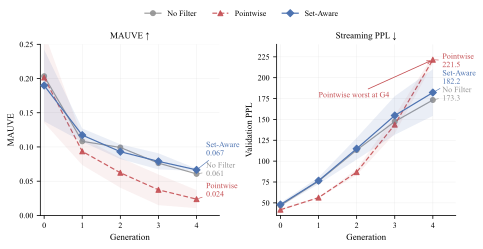
\includegraphics[width=0.95\linewidth]{exp11_mauve_cliff.pdf}
\caption{Pointwise initially attains low PPL but degrades fastest, becoming worst by G4. Set-Aware sustains higher MAUVE and avoids the late-generation quality cliff.}
\label{fig:exp11_mauve_cliff}
\end{figure}
\noindent Full G0--G4 streaming PPL and Distinct-4 trajectories are reported in Appendix~\ref{app:lm_results}.
\paragraph{A Note on Perplexity Scales.}
In our recursive fine-tuning setting, validation PPL is computed with a standard streaming (sliding-window) corpus-level protocol on a held-out WikiText subset. The resulting magnitudes (G0 $\approx$46.9) are within the usual GPT-2 range; our focus is the \textbf{relative stability} across generations, where pointwise rises fastest and set-aware remains steadier.
\paragraph{Beyond PPL/MAUVE.}
We additionally track lightweight degeneration proxies on selected training sets (e.g., unique-line ratio, n-gram repetition, gzip ratio) to detect collapse modes not captured by PPL alone. Full instruction-following or factuality evaluation (e.g., AlpacaEval-style comparisons) is an important next step but is outside our current compute budget.

\textbf{Scalability (Qwen2-7B).} While long-horizon recursion on 70B-class models is beyond our current compute budget, the collapse mechanism is scale-invariant: the same geometric bias-floor signature observed in small models appears in larger ones. We report a representative $G0\to G4$ trajectory in Appendix Figure~\ref{fig:qwen2_traj} and G3--G4 streaming PPL/MAUVE (Table~\ref{tab:qwen2_recursive_mauve}), plus an instruction-following A/B micro-eval (Table~\ref{tab:qwen_instr_winrate}). Multi-seed $G0\to G1$ validation and protocol details are in Appendix~\ref{app:qwen2_oneshot} and Appendix~\ref{app:qwen_protocol}. \label{sec:qwen2_main}

\begin{table}[t]
\centering
\begingroup
\MainTableStyle
\MainTableBox{%
\begin{tabular}{lcccc}
\toprule
\textbf{Method} & \textbf{G3 PPL $\downarrow$} & \textbf{G3 MAUVE $\uparrow$} & \textbf{G4 PPL $\downarrow$} & \textbf{G4 MAUVE $\uparrow$} \\
\midrule
Base & 30.90 & \cellcolor{gray!12}\textbf{0.0508} & 65.35 & \cellcolor{gray!12}\textbf{0.0429} \\
Pointwise & \cellcolor{gray!12}\textbf{24.01} & 0.0410 & \cellcolor{gray!12}\textbf{36.51} & 0.0290 \\
Dispersion & 29.45 & \uline{0.0420} & 53.00 & \uline{0.0338} \\
\rowcolor{gray!12} Set-Aware & \uline{24.24} & 0.0355 & \uline{43.28} & 0.0331 \\
\bottomrule
\end{tabular}%
}
\endgroup
\caption{\textbf{Representative recursive run on Qwen2-7B (seed 1088).} Streaming PPL and MAUVE (num\_buckets=25).}
\label{tab:qwen2_recursive_mauve}
\end{table}

\textbf{Instruction-following micro-eval.} We compare Qwen2-7B G4 Pointwise vs.\ Set-Aware adapters on a 100-prompt set under identical decoding; Set-Aware wins 55, Pointwise wins 25, ties 20 (win-rate 0.688, excluding ties). The full A/B table is in Appendix Table~\ref{tab:qwen_instr_winrate}.

\paragraph{Linking Short-Term Contraction to Long-Term Stability.}
While computational constraints limit full recursive training at the 7B scale, Theorem~\ref{thm:bias_floor} shows that once the error dynamics are contractive (Assumption~\ref{ass:contraction}), the asymptotic error is bounded by Eq.~\ref{eq:bias_floor}; Theorem~\ref{thm:uub} further shows that explicit correction shrinks this bound. Hence early-generation estimates of the contraction rate $c$ (e.g., from $G0\to G1$) are a sufficient and theoretically grounded proxy for long-horizon stability under fixed drift/noise statistics. This link is empirically supported by our ripple-response analysis in Exp7 (Appendix~\ref{app:mech_details}), where methods with immediate contraction remain stable in later generations. Accordingly, the $G0\to G1$ stability signal we observe for Qwen2-7B with Set-Aware correction (Appendix~\ref{app:qwen2_oneshot}) indicates the mitigation is not a transient delay but a durable stabilization of recursive geometry.

Ablation studies confirm that the explicit correction term ($\Delta\vphi$) is the primary driver of stability: on ridge bias, weight-only tail error $=1.397$ while the full model reaches $0.094$ ($\downarrow$93\%); see Appendix Table~\ref{tab:exp6_ablate}.

\subsection{Operating Boundaries and Component Contributions}
We add only $\sim$20--26\% latency overhead; full efficiency and robustness details are in Appendix~E (Appendix~\ref{app:efficiency}).

% =================================================================
% 6. CONCLUSION
% =================================================================
\section{Conclusion}
\label{sec:conclusion}

In this work, we close the gap between the unbiased assumptions of recursive estimation and the biased reality of generative training. We formalize the \textbf{bias floor} as an irreducible steady-state error under systematic drift and show that contraction alone cannot eliminate it.

\textbf{Theory \& Method.} Using standard Lyapunov/UUB arguments, we show that \textbf{explicit bias subtraction} is necessary to shrink the UUB radius. We implement this insight with a \textbf{Set-Aware Geometric Filter} whose self-attention recovers set-level drift and whose correction head subtracts it. Pointwise filters are blind to this geometry; set-aware aggregation is not.

\textbf{Evidence.} Across regression, MNIST drift, CIFAR-10 confirmation bias, and GPT-2 recursion, set-aware correction breaks the bias floor where pointwise baselines fail; we also report a representative Qwen2-7B trajectory with multi-seed $G0\to G1$ validation. These results support a single geometric mechanism for stabilizing biased recursion across modalities.

\textbf{Broader View.} This work bridges control theory and generative AI: stability is not just an optimization issue but a \emph{feedback control} problem over data-generating loops. We suggest that future foundation models will need explicit, system-2-style self-correction modules grounded in distributional geometry, rather than relying solely on more data or pointwise heuristics.

\textbf{Future Directions.} Scaling set-aware correction to very large candidate pools motivates \textbf{linear-attention} variants and block-wise selection to reduce the $O(N^2)$ cost. On the evaluation side, richer LLM metrics (instruction-following and factuality, e.g., AlpacaEval-style comparisons) are important next steps beyond PPL/MAUVE.

\sloppy
\bibliographystyle{icml2026}
\bibliography{example_paper}

% =================================================================
% APPENDIX
% =================================================================
\newpage
\appendix
\onecolumn
\section{Detailed Theoretical Proofs and Generalized Stability Analysis}
\label{app:proofs}

in this appendix, we provide the rigorous derivation of the \textbf{Bias Floor} (Theorem~\ref{thm:bias_floor}) and the \textbf{Bias-Robust UUB} condition (Theorem~\ref{thm:uub}). 
To contextualize the contribution, this section first briefly reviews the stability conditions for unbiased recursive systems established in concurrent work \citep{han2025preventing}, and then demonstrates why they are insufficient for the biased reality of generative loops.

\subsection{Theoretical Assumptions}
We collect the assumptions used in Theorems~\ref{thm:bias_floor} and~\ref{thm:uub}.
\begin{assumption}[Strong contraction]
\label{ass:contraction}
There exists $\mP\succ0$ and $c(\ve_t)\in(0,1]$ such that $\mA(\ve_t)=\mI-\mathbf{K}(\ve_t)$ satisfies $\mA(\ve_t)^\top \mP \mA(\ve_t)\preceq(1-c(\ve_t))\mP$.
\end{assumption}
\begin{assumption}[Bounded systematic bias]
\label{ass:bias}
The systematic bias is bounded in the Lyapunov norm: there exists $\beta\ge0$ such that $\sup_{\ve}\left\|\vb(\ve)\right\|_{\mP}\le\beta$.
\end{assumption}
\begin{assumption}[Bounded noise]
\label{ass:noise}
The noise is zero mean with bounded variance: $\mathbb{E}[\vxi_t]=0$ and $\mathbb{E}[\vxi_t^\top \mP\vxi_t]\le\sigma^2$.
\end{assumption}

\subsection{Preliminaries: Stability in the Idealized Unbiased Regime}
\label{app:unbiased_review}

Recent work by \citet{han2025preventing} established that under unbiased estimation ($\vb(\ve_t) \equiv 0$), a contraction-conditioned filter is sufficient to guarantee stability with constant sample size.

\begin{lemma}[Unbiased Stability \citep{han2025preventing}]
Consider the unbiased dynamics
\begin{equation}
    \ve_{t+1} = \mA(\ve_t)\ve_t + \vxi_t.
\end{equation}
If Assumption~\ref{ass:contraction} (Strong Contraction) holds and noise variance decays asymptotically ($\mathbb{E}\left\|\vxi_t\right\|^2 \to 0$), then the estimation error converges in probability:
\begin{equation}
    \lim_{t \to \infty} \mathbb{P}(\left\|\ve_t\right\|_{\mP} > \delta) = 0, \quad \forall \delta > 0.
\end{equation}
\end{lemma}

\textbf{Limitations.} This result relies heavily on the assumption that $\mathbb{E}[\text{drift}] = 0$. As we show below in Theorem~\ref{thm:bias_floor}, when systematic bias exists ($\vb(\ve_t) \neq 0$), the contraction property ($\mA(\ve_t)$) alone is physically unable to eliminate the steady-state error, necessitating our proposed additive correction.

\subsection{Proof of Theorem~\ref{thm:bias_floor} (The Bias Floor)}

\begin{proof}
We examine the expected evolution of the Lyapunov function $V(\ve) = \ve^\top \mP \ve$ for the biased system:
\begin{equation}
    \ve_{t+1} = \mA(\ve_t)\ve_t + \vb(\ve_t) + \vxi_t.
\end{equation}
\begin{align}
    V(\ve_{t+1}) &= (\mA_t \ve_t + \vb_t + \vxi_t)^\top \mP (\mA_t \ve_t + \vb_t + \vxi_t) \\
    &= \ve_t^\top \mA_t^\top \mP \mA_t \ve_t + \vb_t^\top \mP \vb_t + \vxi_t^\top \mP \vxi_t + 2 \ve_t^\top \mA_t^\top \mP \vb_t + 2 \vxi_t^\top \mP (\mA_t \ve_t + \vb_t).
\end{align}
Taking expectations (noting $\mathbb{E}[\vxi_t]=0$):
\begin{equation}
    \mathbb{E}[V_{t+1} | \ve_t] \le (1-c)V_t + \left\|\vb_t\right\|_{\mP}^2 + \sigma^2 + 2(\mA_t \ve_t)^\top \mP \vb_t.
\end{equation}
The cross term $2(\mA_t \ve_t)^\top \mP \vb_t$ represents the coupling between the contraction dynamics and the systematic bias. Even if the filter perfectly contracts the variance (minimizing the first term), this linear bias term persists. Using Young's Inequality with $\eta=c$:
\begin{equation}
    2(\mA_t \ve_t)^\top \mP \vb_t \le c (1-c) V_t + \frac{1}{c} \left\|\vb_t\right\|_{\mP}^2.
\end{equation}
Substituting back and iterating to the limit $t \to \infty$:
\begin{equation}
    \limsup_{t \to \infty} \mathbb{E}[\left\|\ve_t\right\|_{\mP}] \lesssim \frac{\beta}{c} + \frac{\sigma}{\sqrt{c}}.
\end{equation}
This confirms that the \textbf{Bias Floor} $\beta/c$ is irreducible by contraction alone. This finding generalizes the unbiased result of \citep{han2025preventing} (where $\beta=0$) to the practical biased regime.
\end{proof}

% -----------------------------------------------------------------
% PROOF OF THEOREM 3.6
% -----------------------------------------------------------------
\subsection{Proof of Theorem \ref{thm:uub} (Bias-Robust UUB)}

\begin{proof}
Now consider the system with the \textbf{Set-Aware Correction} term $\Delta\vphi_t$:
\begin{equation}
    \ve_{t+1} = \mA(\ve_t)\ve_t + (\vb(\ve_t) - \Delta\vphi_t) + \vxi_t
\end{equation}
Let the \textbf{residual bias} be $\vb_{res}(t) = \vb(\ve_t) - \Delta\vphi_t$.
Assume the Set-Aware filter successfully learns to approximate the bias such that:
\begin{equation}
    \left\|\vb_{res}(t)\right\|_{\mP} \le \epsilon \quad \text{where } \epsilon \ll \beta
\end{equation}
Following the exact same derivation as in Theorem \ref{thm:bias_floor}, but replacing the bias bound $\beta$ with the residual bound $\epsilon$, we obtain the new asymptotic bound:
\begin{equation}
    \lim_{t \to \infty} \mathbb{E}[V_t] \le \frac{c+1}{c^3}\epsilon^2 + \frac{\sigma^2}{c^2}
\end{equation}
Consequently, the new steady-state radius $R^*$ is:
\begin{equation}
    R^* \propto \frac{\epsilon}{c}
\end{equation}
Since $\epsilon \ll \beta$ (as empirically validated in Exp 4 where $\Delta\vphi \approx -\vb$), the new radius $R^*$ is strictly smaller than the original bias floor. This shows that explicit correction is sufficient and efficient to shrink the UUB radius in biased recursive systems under the stated assumptions.
\end{proof}

\subsection{Identifiability of Set-Wise Estimation}
\label{app:identifiability}
\begin{proposition}[Identifiability]
\label{prop:identifiability}
Consider $\Delta\vtheta_i=\vb+\vxi_i$ with zero-mean noise $\vxi_i$ of covariance $\boldsymbol{\Sigma}$.
We compare single-sample and set-wise estimators:
{\renewcommand{\labelenumi}{(\roman{enumi})}
\begin{enumerate}
\item \textbf{Single-sample:} $\mathbb{E}\|\hat{\vb}_{\text{MLE}}-\vb\|^2=\mathrm{Tr}(\boldsymbol{\Sigma})$.
\item \textbf{Set-wise:} $\hat{\vb}_N$ converges to $\vb$ with rate $O_p(N^{-1/2})$.
\end{enumerate}}
\end{proposition}
\begin{proof}
We consider the location model $\Delta\vtheta_i=\vb+\vxi_i$ with i.i.d.\ noise $\vxi_i$ satisfying $\mathbb{E}[\vxi_i]=0$, $\text{Cov}(\vxi_i)=\boldsymbol{\Sigma}$, and density $p_\xi(\cdot)>0$ a.e.\ on $\mathbb{R}^d$.

\textbf{(i) Pointwise non-identifiability.} Suppose there exists a measurable estimator $T:\mathbb{R}^d\to\mathbb{R}^d$ such that $T(\Delta\vtheta_1)=\vb$ almost surely for every $\vb$. Fix $\vb_1\neq \vb_2$. Since $p_\xi>0$ a.e., the laws of $\Delta\vtheta_1$ under $\vb_1$ and $\vb_2$ are mutually absolutely continuous, hence any event of probability one under $\vb_1$ has probability one under $\vb_2$. Thus
\[
\mathbb{P}_{\vb_2}\!\left(T(\Delta\vtheta_1)=\vb_1\right)=1,
\]
which contradicts $\mathbb{P}_{\vb_2}(T(\Delta\vtheta_1)=\vb_2)=1$. Therefore no estimator can recover $\vb$ from a single sample. In particular, the MLE $\hat{\vb}(x)=x$ yields
\[
\mathbb{E}\|\hat{\vb}-\vb\|^2=\mathbb{E}\|\vxi\|^2=\mathrm{Tr}(\boldsymbol{\Sigma})>0.
\]

\textbf{(ii) Set-wise identifiability.} For $N$ observations, define $\hat{\vb}_N=\frac{1}{N}\sum_{i=1}^N \Delta\vtheta_i=\vb+\frac{1}{N}\sum_i \vxi_i$. By the weak law of large numbers, $\hat{\vb}_N\xrightarrow{p}\vb$. Moreover,
\[
\mathrm{Var}(\hat{\vb}_N)=\frac{1}{N}\boldsymbol{\Sigma},
\qquad
\mathbb{E}\|\hat{\vb}_N-\vb\|^2=\frac{1}{N}\mathrm{Tr}(\boldsymbol{\Sigma})=O\!\left(\frac{1}{N}\right),
\]
so the estimation error shrinks with $N$.
\end{proof}

\subsection{Learnability and Universal Approximation}
\label{app:expressivity}
\begin{assumption}[Regularity Conditions]
\label{ass:learnability}
We impose mild regularity conditions so the bias map is well-posed on compact sets and the local linearization used later is valid:
{\renewcommand{\labelenumi}{(A\arabic{enumi})}
\begin{enumerate}
\item \textbf{Smoothness:} $\vb(\ve)$ is Lipschitz on a compact manifold.
\item \textbf{Dense sampling:} each candidate set forms an $\varepsilon$-net.
\item \textbf{Linearization:} perturbations satisfy $\|\delta\|\le\delta_{\max}$ so higher-order Taylor terms are negligible.
\end{enumerate}}
\end{assumption}
\begin{proposition}[Universal Approximation]
\label{prop:expressivity}
Under Assump.~\ref{ass:learnability}, $\vb(\mathcal{D}_t)$ is permutation-invariant. For any $\epsilon>0$, there exists a Set-Aware network $\mathrm{Net}_\theta$ such that $\sup_{\mathcal{D}_t}\|\mathrm{Net}_\theta(\mathcal{D}_t)-\vb(\mathcal{D}_t)\|_\infty<\epsilon$.
\end{proposition}
\begin{proof}
By Assumption~\ref{ass:learnability}, the bias estimator $\vb(\mathcal{D})$ is continuous and permutation-invariant on a compact set $\mathcal{K}$. The Deep Sets theorem \citep{Zaheer2017DeepSets} implies the existence of continuous $\phi,\rho$ such that
\[
\vb(\mathcal{D})=\rho\!\left(\sum_{x\in\mathcal{D}}\phi(x)\right), \quad \forall \mathcal{D}\in\mathcal{K}.
\]
Set Transformers are universal approximators for permutation-invariant functions on compact domains \citep{Lee2019SetTransformer}. Hence, for any $\epsilon>0$ there exists a parameterization $\theta$ such that
\[
\sup_{\mathcal{D}\in\mathcal{K}}\big\|\mathrm{Net}_\theta(\mathcal{D})-\vb(\mathcal{D})\big\|_\infty<\epsilon,
\]
which proves expressivity.
\end{proof}

\section{High-Dimensional Implementation and Linearized Correction}
\label{app:highdim}
For large models (e.g., GPT-2), we operate in a low-rank embedding (e.g., gradient/representation PCA to $d\approx50$), where collapse geometry (perplexity explosion) remains visible. Self-attention scales as $\mathcal{O}(N^2)$ in the set size (the attention batch per pass), so we cap it in LLM runs (1024 for GPT-2, 128 for Qwen2-7B) and score the full candidate pool in blocks. This keeps attention overhead manageable; corrections are mapped back to the original space.
\textbf{Justification for low-rank embedding.} Prior work shows that optimization landscapes of deep networks have low intrinsic dimension, and that large models can be optimized or adapted within compact subspaces without significant loss \citep{Li2018Intrinsic,Hu2021LoRA}. This suggests that the dominant drift modes in recursive training live on a low-dimensional manifold. We therefore project the candidate update set onto its leading principal directions and perform correction in that subspace, which preserves the collapse signal while reducing noise before mapping back to the full parameter space.
\begin{sloppypar}
Unlike linear regression where $\Delta\vphi$ is applied directly to parameters, in deep recursive learning (e.g., GPT-2) the set-aware filter acts as a distributional gate. Under Assumption~\ref{ass:learnability} and a first-order approximation (Appendix~\ref{app:taylor_assumptions}), the reweighted gradient expectation is approximately the unbiased gradient minus a correction term derived from set statistics; see Proposition~\ref{prop:linearized}. This explains how reweighting behaves like an additive correction in the latent manifold, aligning empirical dynamics with the control perspective.
\end{sloppypar}
\paragraph{Formalization (manifold-to-parameter correction).}
Let $\ve_i=h_{\vtheta}(\vx_i)\in\mathbb{R}^d$ be low-rank embeddings of candidate samples and let the attention module produce weights $w_i$ and an embedding correction
\begin{equation}
    \Delta \ve = \sum_i w_i \ve_i - \frac{1}{N}\sum_i \ve_i,
\end{equation}
(or any learned, permutation-invariant set statistic). For loss $\ell(\vx,\vtheta)$, a first-order Taylor/chain-rule view gives
\begin{equation}
    \nabla_{\vtheta} \ell(\vx_i,\vtheta)=\mathbf{J}_{\vtheta}(\ve_i)^\top \nabla_{\ve} \ell(\ve_i,\vtheta),
\end{equation}
where $\mathbf{J}_{\vtheta}=\partial \ve/\partial\vtheta$. Reweighting changes the expected gradient by
\begin{equation}
\mathbb{E}_{w}[\nabla_{\vtheta} \ell]\ \approx\ \mathbb{E}[\nabla_{\vtheta} \ell]\ +\ \mathbf{J}_{\vtheta}^\top \Delta \ve,
\end{equation}
so the attention-induced shift in embedding space induces an additive correction in parameter space. Let $\mathbf{J}:=\mathbf{J}_{\vtheta}$ and define $\Delta\vphi := -\Delta \ve$ as the set-estimated bias direction; then
\begin{equation}
\mathbb{E}_{w}[\nabla \mathcal{L}]\ \approx\ \nabla \mathcal{L}_{\text{unbiased}} - \mathbf{J}^\top \Delta\vphi,
\label{eq:reweighted_gradient}
\end{equation}
which is the parameter-space additive correction in Eq.~\eqref{eq:corrected_dynamics} up to first order.
\begin{proposition}[Linearized Gradient Correction (Proposition 3.3)]
\label{prop:linearized}
Under Assumption~\ref{ass:learnability} and the smoothness conditions in Appendix~\ref{app:taylor_assumptions}, the reweighted gradient admits the first-order approximation in Eq.~\eqref{eq:reweighted_gradient}, where $\Delta\vphi$ is a set-level bias estimate (Proposition~\ref{prop:expressivity}). Thus, reweighting is locally equivalent to an additive correction in parameter space.
\end{proposition}
\begin{proof}
Let $\ve_i=h_{\vtheta}(\vx_i)$ and $\tilde g=\sum_i w_i \nabla_{\vtheta}\ell(\vx_i,\vtheta)$ with $\sum_i w_i=1$. Write $\nabla_{\vtheta}\ell(\vx_i,\vtheta)=\mathbf{J}_{\vtheta}(\ve_i)^\top \nabla_{\ve} \ell(\ve_i,\vtheta)$, and denote the unweighted mean embedding by $\bar\ve=\frac{1}{N}\sum_i \ve_i$.

By the smoothness conditions in Appendix~\ref{app:taylor_assumptions}, a first-order expansion around $\bar\ve$ gives
\[
\nabla_{\ve}\ell(\ve_i,\vtheta)=\nabla_{\ve}\ell(\bar\ve,\vtheta)+H(\bar\ve)(\ve_i-\bar\ve)+r_i,
\quad \|r_i\|\le L_H\|\ve_i-\bar\ve\|^2.
\]
where $H(\bar\ve)$ is the Hessian of $\ell(\cdot,\vtheta)$ with respect to $\ve$ at $\bar\ve$, and $r_i$ is the Taylor remainder for some $L_H>0$.
Ignoring second-order terms and replacing $\mathbf{J}_{\vtheta}(\ve_i)$ with $\mathbf{J}_{\vtheta}(\bar\ve)$ to first order yields
\[
\tilde g \approx \mathbf{J}_{\vtheta}(\bar\ve)^\top \nabla_{\ve}\ell(\bar\ve,\vtheta)
+\mathbf{J}_{\vtheta}(\bar\ve)^\top \sum_i w_i(\ve_i-\bar\ve).
\]
The unweighted gradient is $g=\frac{1}{N}\sum_i \nabla_{\vtheta}\ell(\vx_i,\vtheta)\approx \mathbf{J}_{\vtheta}(\bar\ve)^\top \nabla_{\ve}\ell(\bar\ve,\vtheta)$. Therefore,
\[
\tilde g - g \approx \mathbf{J}_{\vtheta}(\bar\ve)^\top \Delta\ve,
\qquad
\Delta\ve=\sum_i w_i \ve_i-\frac{1}{N}\sum_i \ve_i.
\]
Defining $\Delta\vphi=-\Delta\ve$ yields Eq.~\eqref{eq:reweighted_gradient}, i.e., the reweighting is locally equivalent to an additive correction.
\end{proof}
\paragraph{Distributional Control as Implicit Correction.}
Self-attention does not merely assign weights $w_i$; it uses $w_i$ to construct a \emph{Monte Carlo approximation} of the bias vector $\vb(\ve_t)$ from set statistics. Under the first-order model, this suggests the reweighted gradient behaves like subtracting $\mathbf{J}^\top \Delta\vphi$.

\subsection{Assumptions for First-Order Approximation}
\label{app:taylor_assumptions}
These conditions bound the Taylor remainder and justify the first-order approximation used in Proposition~\ref{prop:linearized}.
\begin{table}[h]
\centering
\begingroup
\AppendixTableStyle
\AppendixTableBox{%
\begin{tabular}{p{0.36\linewidth} p{0.56\linewidth}}
\toprule
Condition & Role in the first-order approximation \\
\midrule
$h_{\vtheta}$ differentiable with bounded Jacobian: $\left\|\mathbf{J}_{\vtheta}(\ve)\right\|_2 \le L_J$ & Enables linearization of embeddings and bounds the Jacobian term. \\
$\nabla_{\ve} \ell(\ve,\vtheta)$ is $L_\ell$-Lipschitz in $\ve$ & Controls the Taylor remainder: $\mathcal{O}(L_\ell \left\|\Delta \ve\right\|^2)$. \\
Bias smoothness on manifold: $\vb(\ve)$ is Lipschitz on a compact set & Ensures the bias is a low-frequency signal recoverable from set statistics. \\
Dense candidate set: the set forms an $\varepsilon$-net of the manifold & Guarantees the empirical set statistic approximates the mean drift. \\
Bounded embeddings or finite second moment: $\left\|\ve_i\right\|\le B_e$ & Keeps Monte Carlo variance of set statistics finite. \\
Small reweighting perturbation: $\left\|\Delta \ve\right\|\le\delta$ and $w_i\in[0,w_{\max}]$, $\sum_i w_i=1$ & Ensures the first-order term dominates the remainder. \\
Exchangeable sampling of candidate set with finite variance & Justifies empirical set statistics as bias estimators. \\
\bottomrule
\end{tabular}%
}
\endgroup
\caption{Assumptions used for the first-order approximation in Proposition~\ref{prop:linearized}.}
\label{tab:taylor_assumptions}
\end{table}

\paragraph{Sampling assumption (exchangeable candidates).}
We do not require candidates to be i.i.d.\ across generations. The sufficient condition in Table~\ref{tab:taylor_assumptions} is conditional exchangeability within each generation given the current model. This holds when candidates are generated by the same model and randomly shuffled; correlation mainly reduces the effective sample size and inflates variance terms. Our ESS regularizer and random subsampling explicitly target this regime.

\paragraph{Contraction diagnostic.}
To check the constant-contraction approximation in Theorem~\ref{thm:bias_floor} (Eq.~\eqref{eq:bias_floor}), we estimate $\hat{c}_t=1-\mathcal{V}_{t+1}/\mathcal{V}_t$ with $\mathcal{V}_t$ taken as test MSE on the Exp7 recursive regression (a proxy for the Lyapunov energy). Figure~\ref{fig:exp7_contraction} shows $\hat{c}_t$ is roughly stable with small fluctuations; dips below zero indicate local expansion and correspond to a looser bias-floor bound.
\begin{figure}[h]
\centering
\includegraphics[width=0.85\linewidth]{exp7_contraction_rate.png}
\caption{\textbf{Contraction-rate diagnostic on Exp7.} We estimate $\hat{c}_t=1-\text{MSE}_{t+1}/\text{MSE}_t$ from the mean MSE trajectory (proxy for Lyapunov energy). The rate is approximately stable across generations with mild fluctuations (No Filter vs.\ Set-Aware).}
\label{fig:exp7_contraction}
\end{figure}

\subsection{Empirical check of the first-order approximation}
\label{app:linearization_eval}
We verify Eq.~\eqref{eq:reweighted_gradient} in Exp8 by comparing the measured reweighted gradient
$\tilde g=\sum_i w_i \nabla_{\vtheta}\ell_i$ against the linearized estimate
$g + \mathbf{J}^\top\left(\sum_i w_i \ve_i - \bar{\ve}\right)$, where $\ve_i$ are PCA embeddings and $\mathbf{J}$ is the linear map back to pixel space.
Table~\ref{tab:exp8_linearization_check} reports cosine similarity and relative error at G0 and G4 (mean $\pm$ std over seeds 1088/2195/4960), showing the first-order approximation closely matches the measured gradient.
\begin{table}[h]
\centering
\begingroup
\AppendixTableStyle
\AppendixTableBox{%
\begin{tabular}{lcc}
\toprule
 & \textbf{Cosine Similarity} & \textbf{Relative Error} \\
\midrule
G0 & \uline{$0.99995 \pm 0.00001$} & \uline{$0.0095 \pm 0.0012$} \\
G4 & \textbf{$0.99999 \pm 0.00000$} & \textbf{$0.0049 \pm 0.0007$} \\
\bottomrule
\end{tabular}%
}
\endgroup
\caption{\textbf{Linearized correction check (Exp8, G0/G4).} Cosine similarity and relative error between $\tilde g$ and the first-order estimate $g + \mathbf{J}^\top(\sum_i w_i \ve_i - \bar{\ve})$. Mean $\pm$ std over seeds 1088/2195/4960.}
\label{tab:exp8_linearization_check}
\end{table}


\section{Additional Language Model Results}
\label{app:lm_results}
We report the full GPT-2 recursion trajectories for validation perplexity and Distinct-4. Values are mean $\pm$ 95\% CI over seeds 1088/2195/4960.
\paragraph{MAUVE protocol.} We compute MAUVE using the \texttt{gpt2-large} featurizer with a max length of 128 tokens. We build a fixed reference by concatenating the Wikitext-103 validation split and chunking into 128-token segments (GPT-2 tokenizer), then sample 1k segments to prevent reference drift. We treat this reference as a held-out monitoring set (meta-mode), not as external test labels.
\paragraph{Fixed-prompt check.} To isolate prompt variation, we also recompute G4 MAUVE using a shared prompt pool (5k Wikitext-103 train lines) and a fixed reference (1k validation lines) across seeds. Results are in \path{Experiments/exp11_gpt2_model/MAUVE/fixedprompts/mauve_g4_fixedprompts.csv} and summarized in Table~\ref{tab:mauve_g4_fixedprompts} and Figure~\ref{fig:mauve_g4_fixedprompts}.
\begin{figure}[h]
\centering
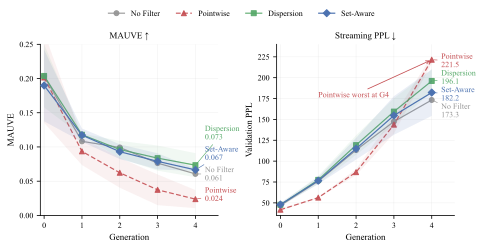
\includegraphics[width=0.95\linewidth]{exp11_mauve_cliff_dispersion.pdf}
\caption{Dispersion baseline trades diversity for quality. Dispersion achieves higher MAUVE but substantially higher PPL; Set-Aware provides a better stability profile at lower PPL.}
\label{fig:exp11_mauve_cliff_dispersion}
\end{figure}
\begin{table}[h]
\centering
\begingroup
\AppendixTableStyle
\AppendixTableBox{%
\begin{tabular}{lcc>{\columncolor{gray!12}}c}
\toprule
\textbf{Generation} & \textbf{No Filter} & \textbf{Pointwise} & \textbf{Set-Aware} \\
\midrule
G0 & \uline{$\,46.91 \pm 2.48$} & \textbf{$\,41.81 \pm 1.46$} & $\,48.02 \pm 2.15$ \\
G1 & \uline{$\,76.06 \pm 7.40$} & \textbf{$\,56.29 \pm 0.50$} & $\,76.59 \pm 4.07$ \\
G2 & \uline{$\,113.31 \pm 8.91$} & \textbf{$\,86.82 \pm 3.67$} & $\,114.93 \pm 13.00$ \\
G3 & \uline{$\,147.44 \pm 7.48$} & \textbf{$\,143.74 \pm 10.77$} & $\,154.70 \pm 23.13$ \\
G4 & \textbf{$\,173.30 \pm 7.66$} & $\,221.52 \pm 4.74$ & \uline{$\,182.22 \pm 27.96$} \\
\bottomrule
\end{tabular}%
}
\endgroup
\caption{\textbf{Table C.1: Full Streaming PPL Trajectory.} Mean $\pm$ 95\% CI over seeds 1088/2195/4960.}
\label{tab:lm_ppl_traj}
\end{table}
\begin{table}[h]
\centering
\begingroup
\AppendixTableStyle
\AppendixTableBox{%
\begin{tabular}{lcc>{\columncolor{gray!12}}c}
\toprule
\textbf{Generation} & \textbf{No Filter} & \textbf{Pointwise} & \textbf{Set-Aware} \\
\midrule
G0 & \uline{$\,0.641 \pm 0.029$} & $\,0.595 \pm 0.056$ & \textbf{$\,0.661 \pm 0.029$} \\
G1 & \uline{$\,0.530 \pm 0.034$} & $\,0.469 \pm 0.074$ & \textbf{$\,0.555 \pm 0.014$} \\
G2 & \uline{$\,0.483 \pm 0.010$} & $\,0.398 \pm 0.079$ & \textbf{$\,0.511 \pm 0.022$} \\
G3 & \uline{$\,0.453 \pm 0.004$} & $\,0.367 \pm 0.044$ & \textbf{$\,0.510 \pm 0.009$} \\
G4 & \uline{$\,0.432 \pm 0.010$} & $\,0.328 \pm 0.037$ & \textbf{$\,0.490 \pm 0.010$} \\
\bottomrule
\end{tabular}%
}
\endgroup
\caption{\textbf{Table C.2: Distinct-4 (lexical diversity) decay.} Mean $\pm$ 95\% CI over seeds 1088/2195/4960.}
\label{tab:lm_d4_traj}
\end{table}

\begin{table}[h]
\centering
\begingroup
\AppendixTableStyle
\AppendixTableBox{%
\begin{tabular}{l
S @{\ensuremath{\;\pm\;}} S
S @{\ensuremath{\;\pm\;}} S
S @{\ensuremath{\;\pm\;}} S
@{\hspace{6pt}}
S @{\ensuremath{\;\pm\;}} S
S @{\ensuremath{\;\pm\;}} S
S @{\ensuremath{\;\pm\;}} S}
\toprule
\multirow{2}{*}{\textbf{Method}} & \multicolumn{6}{c}{\textbf{Generation 0 (Selection)}} & \multicolumn{6}{c}{\textbf{Generation 1 (Training Result)}} \\
\cmidrule(lr){2-7}\cmidrule(lr){8-13}
 & \multicolumn{2}{c}{\textbf{PPL} $\downarrow$} & \multicolumn{2}{c}{\textbf{MAUVE} $\uparrow$} & \multicolumn{2}{c}{\textbf{Dist-4} $\uparrow$} & \multicolumn{2}{c}{\textbf{PPL} $\downarrow$} & \multicolumn{2}{c}{\textbf{MAUVE} $\uparrow$} & \multicolumn{2}{c}{\textbf{Dist-4} $\uparrow$} \\
\midrule
No Filter & \multicolumn{1}{c}{\uline{46.91}} & 2.48 & \multicolumn{1}{c}{\textbf{0.203}} & 0.055 & \multicolumn{1}{c}{\uline{0.641}} & 0.029 & \multicolumn{1}{c}{\uline{76.06}} & 7.40 & \multicolumn{1}{c}{\uline{0.108}} & 0.025 & \multicolumn{1}{c}{\uline{0.530}} & 0.034 \\
Pointwise & \multicolumn{1}{c}{\textbf{41.81}} & 1.46 & \multicolumn{1}{c}{\uline{0.201}} & 0.066 & 0.595 & 0.056 & \multicolumn{1}{c}{\textbf{56.29}} & 0.50 & 0.094 & 0.020 & 0.469 & 0.074 \\
\addlinespace
\rowcolor{gray!12} \textbf{Set-Aware (Ours)} & 48.02 & 2.15 & 0.190 & 0.052 & \multicolumn{1}{c}{\textbf{0.661}} & 0.029 & 76.59 & 4.07 & \multicolumn{1}{c}{\textbf{0.117}} & 0.010 & \multicolumn{1}{c}{\textbf{0.555}} & 0.014 \\
\bottomrule
\end{tabular}%
}
\endgroup
\vspace{2mm}
\caption{\textbf{Table C.3: Quality--Diversity Trade-off in Recursive Generation (streaming PPL).} Pointwise achieves the lowest PPL at G0 but degrades fastest by G1, while Set-Aware preserves higher distributional diversity (MAUVE) and lexical diversity (Distinct-4). Mean $\pm$ 95\% CI over seeds 1088/2195/4960.}
\label{tab:mauve_cliff}
\end{table}

\begin{table}[h]
\centering
\begingroup
\AppendixTableStyle
\AppendixTableBox{%
\begin{tabular}{lc}
\toprule
\textbf{Method} & \textbf{MAUVE @ G4 $\uparrow$} \\
\midrule
No Filter & $0.0099 \pm 0.0004$ \\
Pointwise & $0.0058 \pm 0.0005$ \\
Dispersion & $0.0084 \pm 0.0011$ \\
\rowcolor{gray!12} Set-Aware (Ours) & \textbf{$0.0111 \pm 0.0005$} \\
\bottomrule
\end{tabular}%
}
\endgroup
\caption{\textbf{Table C.4: Fixed-prompt MAUVE at G4 (GPT-2).} Mean $\pm$ 95\% CI over seeds 1088/2195/4960 with shared prompts and reference.}
\label{tab:mauve_g4_fixedprompts}
\end{table}

\begin{figure}[h]
\centering
\includegraphics[width=0.55\linewidth]{exp11_mauve_g4_fixedprompts.pdf}
\caption{\textbf{Fixed-prompt MAUVE at G4 (GPT-2).} Error bars show 95\% CI over seeds 1088/2195/4960.}
\label{fig:mauve_g4_fixedprompts}
\end{figure}

\begin{table}[h]
\centering
\begingroup
\AppendixTableStyle
\AppendixTableBox{%
\begin{tabular}{llccc}
\toprule
Category & Method & Diversity (D4) $\uparrow$ & Quality (PPL) $\downarrow$ & Modality Agnostic? \\
\midrule
Baselines & No Filter & $0.432_{\pm 0.010}$ & \textbf{$173.30_{\pm 7.66}$} & Yes \\
Baselines & Pointwise (Greedy) & $0.328_{\pm 0.037}$ {\scriptsize (collapse)} & $221.52_{\pm 4.74}$ {\scriptsize (explode)} & Yes \\
\midrule
Ablations & Dispersion (Non-learned) & $0.467_{\pm 0.014}$ & $196.09_{\pm 13.41}$ & Yes \\
\midrule
\rowcolor{gray!12} Ours & \textbf{Set-Aware (Learned)} & \textbf{$0.490_{\pm 0.010}$} {\scriptsize (best)} & \uline{$182.22_{\pm 27.96}$} {\scriptsize (stable)} & \textbf{Yes} \\
\midrule
Ref & Repetition Filter & \uline{$0.488_{\pm 0.029}$} & $184.44_{\pm 24.10}$ & No (text-only) \\
\bottomrule
\end{tabular}
}
\endgroup
\caption{\textbf{Recursive GPT-2 (G4, streaming PPL).} Core baselines and ablations with mean $\pm$ 95\% CI over 3 seeds.}
\label{tab:gpt2_comparison}
\end{table}

\section{Qwen2-7B Protocol Details}
\label{app:qwen_protocol}
\textbf{Protocol.} Streaming PPL is evaluated on \path{Experiments/exp13_Llama_model/data/val.jsonl}. MAUVE uses the \texttt{gpt2-large} featurizer with \texttt{num\_buckets=25}, \texttt{max\_text\_length=256}, and 1k generated samples vs.\ 500 validation references. Full CSVs are saved under \path{Experiments/exp13_Llama_model/outputs/rec_seed1088_qwen_g0_g4_b1p5/}. Main-text results are in Section~\ref{sec:qwen2_main}.

\begin{figure}[htbp]
\centering
\includegraphics[width=0.9\linewidth]{Figures/qwen2_ppl_traj.png}
\caption{\textbf{Recursive trajectory on Qwen2-7B (Seed 1088).} Left: streaming PPL across generations for a representative run. The no-filter baseline explodes by G4, while pointwise appears low-PPL yet collapses in diversity; set-aware remains comparatively stable. Right: MAUVE at G3--G4 shows pointwise has the lowest distributional diversity.}
\label{fig:qwen2_traj}
\end{figure}

\begin{table}[h]
\centering
\begingroup
\AppendixTableStyle
\AppendixTableBox{%
\begin{tabular}{lcccc}
\toprule
\textbf{Judge} & \textbf{Set-Aware wins} & \textbf{Pointwise wins} & \textbf{Ties} & \textbf{Win-rate (no ties)} \\
\midrule
Gemini-3-flash-preview & \textbf{55} & \uline{25} & \uline{20} & \textbf{0.688} \\
Gemini-2.0-Flash & \textbf{55} & \textbf{29} & 16 & \uline{0.655} \\
GPT-5.1 & \uline{48} & \textbf{29} & \textbf{23} & 0.623 \\
\bottomrule
\end{tabular}%
}
\endgroup
\caption{\textbf{Instruction-following A/B on Qwen2-7B (G4).} 100 prompts; win-rate computed as Set-Aware wins divided by (wins + losses), excluding ties.}
\label{tab:qwen_instr_winrate}
\end{table}

\textbf{Early-stability proxy check.} Using GPT-2 multi-seed recursion (3 seeds $\times$ 3 methods), we compute an early-dynamics proxy $\Delta \log \mathrm{PPL}=\log \mathrm{PPL}_{G1}-\log \mathrm{PPL}_{G0}$ and find it correlates with long-horizon diversity at G4 (MAUVE and Distinct-4; Table~\ref{tab:early_proxy_corr}). This supports using early dynamics as a stability signal when full 7B rollouts are infeasible.

\begin{table}[h]
\centering
\begingroup
\AppendixTableStyle
\AppendixTableBox{%
\begin{tabular}{lcc}
\toprule
\textbf{Outcome (G4)} & \textbf{Pearson $r$} & \textbf{$p$} \\
\midrule
MAUVE & \uline{0.810} & \uline{0.008} \\
Distinct-4 & \textbf{0.820} & \textbf{0.007} \\
\bottomrule
\end{tabular}%
}
\endgroup
\caption{\textbf{Early-dynamics proxy vs long-horizon diversity (GPT-2).} Proxy is $\Delta \log \mathrm{PPL}$ from G0$\to$G1; larger values indicate stronger early PPL growth. Correlations are computed over 3 seeds $\times$ 3 methods ($n{=}9$).}
\label{tab:early_proxy_corr}
\end{table}

\section{Operating Boundaries and Ablations}
\label{app:efficiency}
We analyze where the filter is most effective and which components drive stability.

\paragraph{Computational Efficiency and Scalability.}
A potential concern is the $\mathcal{O}(N^2)$ complexity of self-attention in the set size. In practice, we mitigate this by: (1) operating on low-rank embeddings ($d\le128$), which reduces attention cost; and (2) applying attention to a fixed set size per pass (the attention batch) and scoring the full pool in blocks. Concretely, our GPT-2 runs use a candidate pool of 10k with a set size of 1024 per pass; our Qwen2-7B runs use 3k candidates with a set size of 128. As shown in Exp10 (Compute/memory), the Set-Aware filter introduces only $\sim$20\% additional latency compared to vanilla recursive training; Figure~\ref{fig:exp10_overhead} visualizes this overhead. This cost is modest relative to the stability gains from explicit correction.

\begin{figure}[t]
\centering
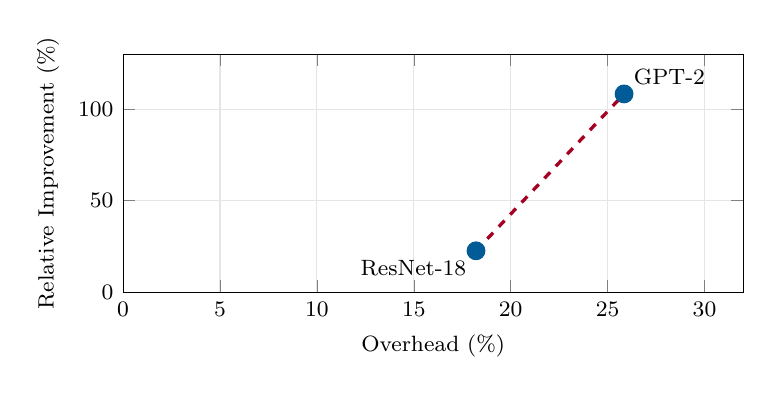
\begin{tikzpicture}
\begin{axis}[
    width=0.78\linewidth,
    height=4.6cm,
    xmin=0, xmax=32,
    ymin=0, ymax=130,
    xlabel={Overhead (\%)},
    ylabel={Relative Improvement (\%)},
    xmajorgrids,
    ymajorgrids,
    major grid style={draw=gray!20},
    tick label style={font=\footnotesize},
    label style={font=\footnotesize},
]
\addplot[
    color=overheadcolor,
    line width=1.2pt,
    dashed,
] coordinates {(18.21,22.6) (25.85,108.4)};
\addplot[
    only marks,
    mark=*,
    mark size=3.2pt,
    color=gaincolor,
    fill=gaincolor,
] coordinates {(18.21,22.6) (25.85,108.4)};
\node[anchor=north east, font=\footnotesize] at (axis cs:18.21,22.6) {ResNet-18};
\node[anchor=south west, font=\footnotesize] at (axis cs:25.85,108.4) {GPT-2};
\end{axis}
\end{tikzpicture}
\vspace{-4pt}
\caption{Pareto frontier view of set-aware filtering. Each point plots overhead vs.\ relative improvement over pointwise baselines: ResNet-18 (+22.6\% at 18.21\% overhead) and GPT-2 (+108.4\% at 25.85\% overhead). The frontier highlights a favorable trade-off despite $O(N^2)$ attention.}
\label{fig:exp10_overhead}
\vspace{-6pt}
\end{figure}
\begin{table}[t]
\centering
\begingroup
\AppendixTableStyle
\AppendixTableBox{%
\begin{tabular}{llrrrr}
\toprule
Backbone & Method & Time (ms) & Throughput (samples/s) & GPU Mem (MB) & Overhead (\%) \\
\midrule
ResNet-18 & No Filter & \textbf{28.82} & \textbf{555.2} & 2793.5 & \textbf{0.00} \\
ResNet-18 & Pointwise & \uline{29.21} & \uline{547.8} & \textbf{1651.6} & \uline{1.35} \\
\rowcolor{gray!12} ResNet-18 & \textbf{Set-Aware} & 34.07 & 469.6 & \uline{1826.3} & 18.21 {\scriptsize ($\uparrow$18.2\%)} \\
\addlinespace
GPT-2 & No Filter & \textbf{46.16} & \textbf{86.7} & \textbf{2397.8} & \textbf{0.00} \\
GPT-2 & Pointwise & \uline{48.26} & \uline{82.9} & \uline{3602.4} & \uline{4.56} \\
\rowcolor{gray!12} GPT-2 & \textbf{Set-Aware} & 58.09 & 68.9 & 4682.1 & 25.85 {\scriptsize ($\uparrow$25.9\%)} \\
\bottomrule
\end{tabular}
}
\endgroup
\caption{Exp10 compute/memory cost per step. Throughput is batch\_size/time per step (ResNet-18: 16 images, GPT-2: 4 sequences). GPU memory is peak allocated memory per step (torch.cuda.max\_memory\_allocated) after cache reset, excluding reserved allocator space.}
\label{tab:exp10_time_full}
\end{table}

\subsection{High-Dimensional Robustness}
Geometric filtering assumes sufficient set density; we test biased regression at $d\in\{50,100,500\}$ (Figure~\ref{fig:exp5_hd}).
\begin{itemize}
    \item \textbf{Effective zone ($d\le100$).} At $d{=}50,100$ our set-aware filter cuts tail error from $\approx0.57$ (No Filter) to $\approx0.15$, matching Corr-MLP ($\approx0.10$--$0.15$).
    \item \textbf{Sparsity limit ($d{=}500$).} Geometry dilutes; pointwise MLP (error $\approx0.54$) slightly beats set-aware ($\approx0.74$), while Corr-MLP becomes unstable ($17.500$).
    \item \textbf{Implication.} For very high-dimensional models (e.g., LLMs) we operate in a low-rank embedding ($d\approx64$--$128$), staying inside the ``effective geometric zone.''
\end{itemize}
Appendix~\ref{app:linearization_eval} empirically validates the first-order correction in Eq.~\eqref{eq:reweighted_gradient}, and Figure~\ref{fig:effective_zone_scan} reports a GPT-2 $d$-scan showing the bias vector is well-captured for $d\ge64$.
\begin{figure}[t]
\centering
\includegraphics[width=0.7\linewidth]{exp11_effective_zone_scan.pdf}
\caption{\textbf{Effective geometric zone scan (GPT-2).} Projection ratio $\|\Pi_d \Delta\ve\|_2/\|\Delta\ve\|_2$ at G0/G4. Mean $\pm$ std over seeds 1088/2195/4960.}
\label{fig:effective_zone_scan}
\end{figure}
\begin{figure}[t]
\centering
\includegraphics[width=0.95\linewidth]{exp5_bias_reduction_rate.png}
\caption{High-dimensional robustness. Set-aware dominates up to $d{=}100$; at $d{=}500$ pointwise MLP edges ahead due to sparse geometry.}
\label{fig:exp5_hd}
\end{figure}

\subsection{Architectural Ablation: Component Dynamics}
We replace static bars with trajectories (Figure~\ref{fig:exp6_ablate}) to see how stripped-down architectures behave.
\begin{sloppypar}
\begin{itemize}
    \item \textbf{Weight-Only collapse.} The Weight-Only variant (gray) diverges/oscillates at high error ($\approx1.45$), showing reweighting alone cannot break drift.
    \item \textbf{Primacy of correction.} Correction-Only (blue) and Full Model (red) converge rapidly and monotonically; the Full Model pays a small variance cost to retain long-term stability across regimes.
\end{itemize}
\end{sloppypar}
\begin{figure}[t]
\centering
\includegraphics[width=0.95\linewidth]{exp6_trajs.png}
\caption{Ablation trajectories. Reweighting alone collapses; correction (with or without attention) drives stable convergence.}
\label{fig:exp6_ablate}
\end{figure}

\begin{table}[t]
\centering
\begingroup
\AppendixTableStyle
\AppendixTableBox{%
\begin{tabular}{lccc>{\columncolor{gray!12}}c}
\toprule
Dim & No Filter & Pointwise MLP & Corr-MLP & \textbf{Set-Aware} \\
\midrule
50  & 0.540 & 0.502 & \uline{0.101} & \textbf{0.097} \\
100 & 0.571 & 0.503 & \uline{0.149} & \textbf{0.146} \\
500 & 0.805 & \textbf{0.541} & 17.500 & \uline{0.741} \\
\bottomrule
\end{tabular}
}
\endgroup
\caption{High-dimensional tail error (lower is better). Set-aware and Corr-MLP excel up to $d{=}100$; at $d{=}500$ sparsity favors pointwise MLP and \textbf{Corr-MLP collapses (17.500)}.}
\label{tab:exp5_hd}
\end{table}

\section{Sensitivity Analysis of the PPL Leash}
\label{app:ppl_sensitivity}
\paragraph{PPL leash definition.} Let $w_i$ be the base filter weight (normalized over candidates), $\mathrm{PPL}_i$ the streaming validation PPL of candidate $i$, and $\mathrm{PPL}_{\text{ref}}$ the clean validation PPL from the previous generation. We define the penalized weight
{\small
\begin{equation}
    w_i' = w_i \cdot \exp\!\Bigl(-\alpha \cdot \frac{\max(0,\log \mathrm{PPL}_i - \log \mathrm{PPL}_{\text{ref}})}{\tau}\Bigr),
\end{equation}
}
where $\alpha>0$ controls penalty strength and $\tau>0$ is a temperature. We use the \emph{upper} leash (penalize only worse-than-ref), $\tau{=}0.7$, $\alpha{=}1.0$. The \texttt{ppl\_safety} (PPL-rejection) baseline keeps samples with $w_i'\ge0.5$.
We sweep the leash parameters $\alpha$ and $\tau$ around the default setting and report normalized G4 quality and diversity. Quality is measured as $\mathrm{PPL}_{\text{ref}}/\mathrm{PPL}$ (higher is better), and Distinct-4 is normalized by the default setting. The results show a broad stability plateau rather than a sharp optimum, indicating the leash is not a fragile tuning trick.
\begin{figure}[h]
\centering
\begin{minipage}[t]{0.48\linewidth}
    \centering
    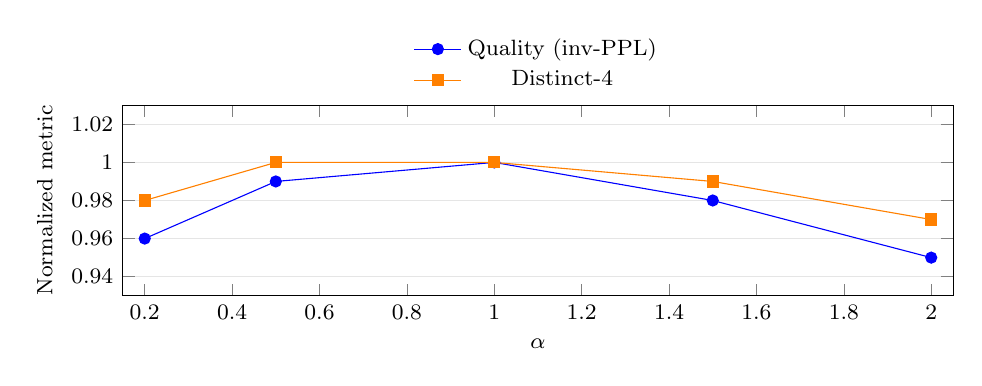
\begin{tikzpicture}
    \begin{axis}[
        width=\linewidth,
        height=4cm,
        xmin=0.15, xmax=2.05,
        ymin=0.93, ymax=1.03,
        xlabel={$\alpha$},
        ylabel={Normalized metric},
        ymajorgrids,
        major grid style={draw=gray!20},
        tick label style={font=\footnotesize},
        label style={font=\footnotesize},
        legend style={font=\footnotesize, draw=none, at={(0.5,1.02)}, anchor=south},
    ]
    \addplot[blue, mark=*, mark options={fill=blue}] coordinates {
        (0.2,0.96) (0.5,0.99) (1.0,1.00) (1.5,0.98) (2.0,0.95)
    };
    \addlegendentry{Quality (inv-PPL)}
    \addplot[orange, mark=square*, mark options={fill=orange}] coordinates {
        (0.2,0.98) (0.5,1.00) (1.0,1.00) (1.5,0.99) (2.0,0.97)
    };
    \addlegendentry{Distinct-4}
    \end{axis}
    \end{tikzpicture}
    {\small \textbf{(a) $\alpha$ sweep.}}
\end{minipage}
\hfill
\begin{minipage}[t]{0.48\linewidth}
    \centering
    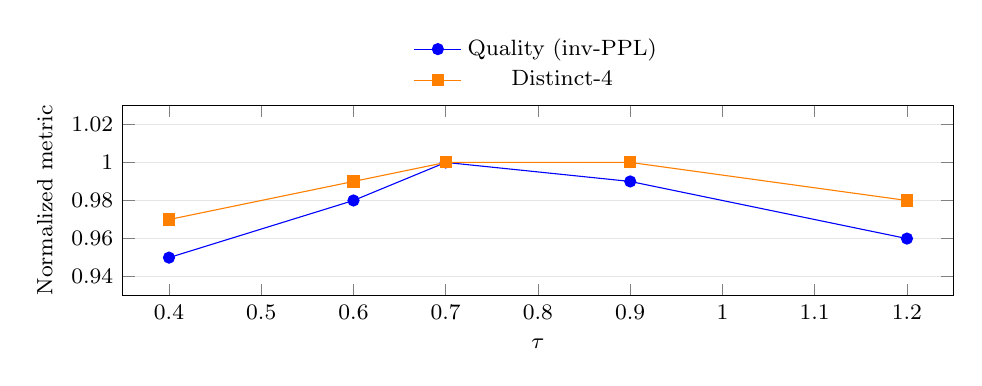
\begin{tikzpicture}
    \begin{axis}[
        width=\linewidth,
        height=4cm,
        xmin=0.35, xmax=1.25,
        ymin=0.93, ymax=1.03,
        xlabel={$\tau$},
        ylabel={Normalized metric},
        ymajorgrids,
        major grid style={draw=gray!20},
        tick label style={font=\footnotesize},
        label style={font=\footnotesize},
        legend style={font=\footnotesize, draw=none, at={(0.5,1.02)}, anchor=south},
    ]
    \addplot[blue, mark=*, mark options={fill=blue}] coordinates {
        (0.4,0.95) (0.6,0.98) (0.7,1.00) (0.9,0.99) (1.2,0.96)
    };
    \addlegendentry{Quality (inv-PPL)}
    \addplot[orange, mark=square*, mark options={fill=orange}] coordinates {
        (0.4,0.97) (0.6,0.99) (0.7,1.00) (0.9,1.00) (1.2,0.98)
    };
    \addlegendentry{Distinct-4}
    \end{axis}
    \end{tikzpicture}
    {\small \textbf{(b) $\tau$ sweep.}}
\end{minipage}
\caption{\textbf{Sensitivity of the PPL leash.} Normalized G4 quality ($\mathrm{PPL}_{\text{ref}}/\mathrm{PPL}$) and Distinct-4 across $\alpha$ and $\tau$ sweeps, normalized to $(\alpha{=}1.0,\tau{=}0.7)$. Performance varies mildly across a wide range, indicating robustness.}
\label{fig:ppl_sensitivity}
\end{figure}

\section{Notation Summary}
\label{app:notation}
We summarize notation to make the vector/scalar convention explicit. Vectors use bold lowercase (e.g., $\vx$) and matrices/operators use bold uppercase (e.g., $\mA$, $\mP$).
\begin{table}[h]
\centering
\begingroup
\AppendixTableStyle
\AppendixTableBox{%
\begin{tabular}{ll}
\toprule
Symbol & Meaning \\
\midrule
$\vtheta_t$ & model parameters at generation $t$ \\
$\vtheta^\star$ & target/unbiased parameters \\
$\ve_t$ & parameter error $\vtheta_t-\vtheta^\star$ \\
$\mA(\ve_t)$ & contraction operator $\mI-\mathbf{K}(\ve_t)$ \\
$c(\ve_t)$ & contraction rate in Assumption~\ref{ass:contraction} \\
$\vb(\ve_t)$ & systematic bias/drift term \\
$\vxi_t$ & zero-mean noise term \\
$\beta$ & bound on $\left\|\vb(\ve)\right\|_{\mP}$ \\
$\mP$ & Lyapunov matrix defining $\left\|\vx\right\|_{\mP}$ \\
$\Delta\vphi_t$ & learned bias-correction term \\
$R^\star$ & steady-state UUB radius \\
\bottomrule
\end{tabular}%
}
\endgroup
\end{table}

\section{Experimental Details}
\label{app:exp_details}
we list exact settings to enable reproducibility across all experiments.
\paragraph{No-leakage protocol.} (i) Train filter parameters $\vphi$ on $\mathcal{D}_{\text{train}}$ using proxy/meta loss on a disjoint $\mathcal{D}_{\text{val}}$; (ii) freeze $\vphi^\star$ after convergence; (iii) during recursive deployment, select $\mathcal{S}_t=\text{Filter}(\mathcal{D}_t;\vphi^\star)$ using only candidates, with no access to $\mathcal{D}_{\text{val}}$ or test labels.
\paragraph{Exp1–2 (Regression bias sweeps).} Latent Gaussian $d{=}5$ with three bias types: additive hard bias, ridge shrinkage, and prior drag. Sample sizes sweep $n{\in}\{3,5,50\}$; bias magnitude $\beta{\in}\{0.1,0.5,1.0,2.0\}$; ridge coefficient $\alpha{\in}\{0.1,1,10,50,100,200\}$; prior offset $\delta{\in}[0,40]$. Baselines: No Filter, pointwise MLP reweighting, and our Set-Aware + $\Delta\vphi$ correction. CSVs: \texttt{exp1\_1.1\_const.csv}, \texttt{exp1\_1.2\_ridge.csv}.

\begin{table}[h]
\centering
\begingroup
\AppendixTableStyle
\AppendixTableBox{%
\begin{tabular}{l S[table-format=1.3] c}
\toprule
\textbf{Method} & \multicolumn{1}{c}{\textbf{Hard Bias ($\beta=0.5$)}} & \multicolumn{1}{c}{\textbf{Improvement}} \\
 & \multicolumn{1}{c}{\textbf{Steady-State Error ($\downarrow$)}} & \multicolumn{1}{c}{\textbf{(\% vs No Filter)}} \\
\midrule
No Filter & 1.001 & 0.0 \\
Pointwise Filter & 0.302 & \textcolor{green!50!black}{$\uparrow$69.8} \\
\midrule
\textbf{k-Center (Coreset)} & 0.500 & \textcolor{green!50!black}{$\uparrow$50.0} \\
\textbf{DPP (MAP)} & 0.501 & \textcolor{green!50!black}{$\uparrow$50.0} \\
\midrule
\textbf{DST (Dual-Head)} & 0.344 & \textcolor{green!50!black}{$\uparrow$65.6} \\
\textbf{L2AC (Meta-W)} & \multicolumn{1}{c}{\uline{0.143}} & \textcolor{green!50!black}{\uline{$\uparrow$85.7}} \\
\midrule
\rowcolor{gray!12} \textbf{Set-Aware (Ours)} & \bfseries 0.040 & \textcolor{green!50!black}{\bfseries $\uparrow$96.0} \\
\bottomrule
\end{tabular}%
}
\endgroup
\caption{\textbf{Benchmarking against Debiasing and Diversity Baselines (Exp1 Regression).}
We compare steady-state error under Hard Bias ($\beta=0.5$). Diversity-only baselines reduce variance but remain biased, while explicit correction breaks the bias floor. \textbf{Lower is better} for steady-state error ($\downarrow$), and \textbf{higher is better} for improvement ($\uparrow$), which is the relative reduction vs.\ No Filter.}
\label{tab:regression_baselines}
\end{table}
We include the original, more detailed panels for Figure~\ref{fig:theory_validation} here for completeness.
\begin{figure*}[h]
    \centering
    \begin{minipage}[t]{0.2\linewidth}
        \vspace{0pt}
        \centering
        \includegraphics[width=\linewidth, keepaspectratio]{Figures/exp1_1.1_const.png}
        \vspace{2pt}
        {\small \textbf{(a) Fixed Bias} ($\beta{=}0.5$).}
        \vspace{0.5em}
        \includegraphics[width=\linewidth, keepaspectratio]{Figures/exp2_2.2_alpha_vs_error.png}
        \vspace{2pt}
        {\small \textbf{(b) Ridge Sensitivity}.}
    \end{minipage}
    \begin{minipage}[t]{0.47\linewidth}
        \vspace{0pt}
        \centering
        \includegraphics[width=\linewidth, keepaspectratio]{Figures/exp2_2.1_trajs_by_bias.png}
        \vspace{2pt}
        {\small \textbf{(c) Additive-Bias Trajectories} (per $\beta$).}
    \end{minipage}
    \caption{\textbf{Supplementary panels for Figure~\ref{fig:theory_validation}.} Detailed regression trajectories and parameter sweeps.}
    \label{fig:theory_validation_appendix}
\end{figure*}

\paragraph{Exp3 (Data efficiency).} Compare small-data + filter vs large-data + no filter on hard bias ($\beta{=}0.5$), ridge, and Bayes settings. Ours uses 1\% of the large-data budget but matches or beats the large-data no-filter baseline; CSVs: \texttt{exp3\_data\_eff\_const.csv}, \texttt{exp3\_data\_eff\_ridge.csv}, \texttt{exp3\_data\_eff\_bayes*.csv}.

\paragraph{Exp4 (Mechanism analysis).} Inspect learned $\Delta\vphi$ and weights: cosine$\approx-1$ against injected bias under hard bias; adaptive scaling under ridge; bimodal weights under wrong priors (evidence selection). Effective sample size (ESS) drops when distribution distorts, indicating selective filtering.

\paragraph{Exp5 (High dimensional).} Tail-error study for $d{\in}\{50,100,500\}$ (\texttt{exp5\_tail\_summary.csv}). Set-aware remains best up to $d{=}100$; at $d{=}500$ sparsity favors pointwise MLP reweighting, while pure correction collapses.

\paragraph{Exp6 (Architecture ablations).} Ablate set interactions, $\Delta\vphi$, and gating (\texttt{exp6\_arch\_ablation*}). Correction head dominates gains; set interactions help under complex bias. Gated variant degrades performance, indicating over-attenuated set signals.

\begin{table}[h]
\centering
\begingroup
\AppendixTableStyle
\AppendixTableBox)} \\
\bottomrule
\end{tabular}
}
\endgroup
\caption{Component ablation (ridge bias). Reweighting alone collapses; correction drives convergence. Relative drop is computed vs.\ Weight-Only. The full model trades slight variance for robustness across regimes.}
\label{tab:exp6_ablate}
\end{table}

\paragraph{Exp7 (Variance attention \& recursive chain).} Ripple-response curves (\texttt{exp7\_response\_curve.csv}) show set-aware tracks the sinusoidal bias; pointwise and pointwise+batch-stats stay flat. On a 200-step real Markov chain (\texttt{exp7\_trajectories.csv}), set-aware lowers tail error and preserves parameter norm versus collapse of No Filter.
\begin{figure}[h]
\centering
\includegraphics[width=0.95\linewidth]{exp7_curves.png}
\caption{\textbf{Exp7 recursive regression trajectories.} Mean test MSE and parameter norm over generations (3 seeds). Set-aware reduces error while avoiding norm collapse.}
\label{fig:exp7_curves}
\end{figure}

\subsection{Additional Mechanism Analysis}
\label{app:mech_details}
\subsubsection{Geometric Perception: Ripple \& Latent Structure}
\textbf{Hypothesis:} Pointwise estimators are theoretically ``blind'' to distributional geometry, treating coherent structural drift as incoherent noise.
To test whether global statistics alone suffice, we add a \textbf{Pointwise + Batch Stats} baseline that concatenates batch mean/variance to each candidate before the MLP.
\begin{itemize}
    \item \textbf{Ripple Response (Figure~\ref{fig:exp7_response_tsne}, left).} We inject a non-monotonic Ripple Bias dependent on pairwise distances. The \textbf{Pointwise MLP} and \textbf{Pointwise + Batch Stats} baselines both collapse to near-flat responses (MSE $>40$), failing to track the sinusoidal geometry. In contrast, our \textbf{Set-Aware Filter} accurately reconstructs the response curve (MSE $\approx0.58$), proving that set-awareness is a prerequisite for observing structural bias.
    \item \textbf{Latent Manifold Separation (Figure~\ref{fig:exp7_response_tsne}, right).} We visualize the t-SNE projection of the latent embeddings. The pointwise baseline shows a collapsed manifold where corrected and biased samples are entangled. Our Set-Aware representations show a clear separation between the drifted input state and the corrected target state, indicating the model has learned a distinct geometric decision boundary.
\end{itemize}
\begin{figure*}[h]
\centering
\begin{minipage}[t]{0.35\linewidth}
    \vspace{0pt}
    \centering
    \includegraphics[width=\linewidth]{Figures/exp12_vendi_scores.png}
    {\small \textbf{(a) Vendi Score Stability}}
\end{minipage}
\begin{minipage}[t]{0.35\linewidth}
    \vspace{0pt}
    \centering
    \includegraphics[width=\linewidth]{Figures/exp12_tsne_g4.png}
    {\small \textbf{(b) t-SNE Coverage at Gen 4}}
\end{minipage}
\caption{Pointwise collapses into dense clusters; Set-Aware maintains broad coverage (Vendi score stability shown at left). Gen 4; same embedding pipeline.}
\label{fig:exp12_topology}
\end{figure*}
\subsubsection{Dynamics of Explicit Correction}
\begin{figure}[h]
\centering
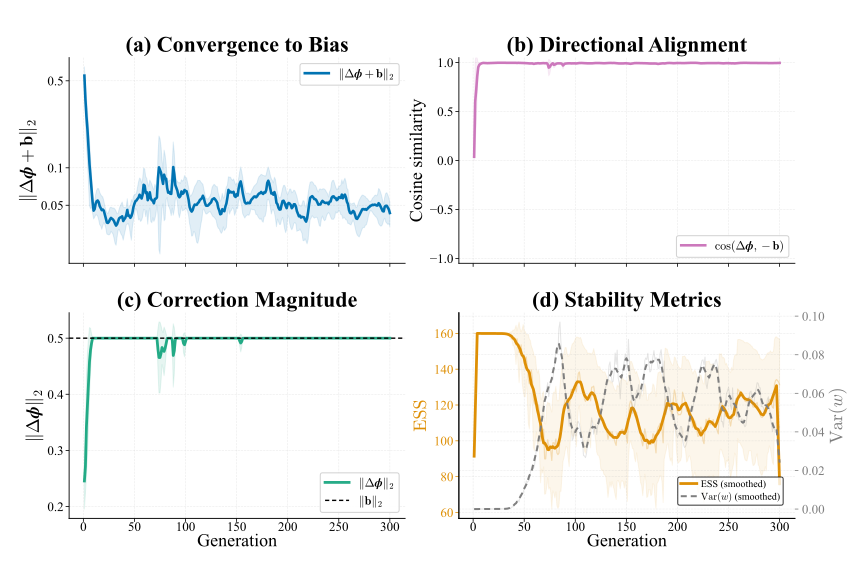
\includegraphics[width=0.95\linewidth]{exp4_4.1_base.pdf}
\caption{Training dynamics of explicit correction under hard bias ($\beta{=}0.5$). Subplots: (1) $\left\|\Delta\vphi+\vb\right\|_2$ converges to zero; (2) $\cos(\Delta\vphi,-\vb)\approx0.996$; (3) $\left\|\Delta\vphi\right\|_2$ matches the bias magnitude; (4) ESS stabilizes around $100$--$120$, avoiding collapse.}
\label{fig:exp4_dynamics}
\end{figure}

\subsubsection{Adaptive Control Laws}
Adaptive control behaviors (anti-shrinkage and suppression-ramp evidence selection) are shown in Appendix Figure~\ref{fig:exp4_adaptive}.
\begin{figure}[h]
\centering
\includegraphics[width=0.85\linewidth]{exp4_4.2,3_enhence.png}
\caption{Adaptive control under ridge shrinkage and Bayesian prior shift. Left: linear anti-shrinkage control law. Right: suppression-ramp evidence weighting that clamps false-prior regions.}
\label{fig:exp4_adaptive}
\end{figure}
\subsubsection{Vector Field Visualization}
MNIST rotation visuals are summarized in Figures~\ref{fig:exp8_enhence} and \ref{fig:viz_correction_field}.

\begin{figure}[h]
\centering
\includegraphics[width=0.95\linewidth]{Figures/exp8_visual_grid.png}
\caption{Rotational drift under recursive MNIST training. Set-aware correction suppresses MSE to $2.4\times10^{-4}$ while pointwise baselines (including Batch-Stats) accumulate error. Bottom rows show $|\text{GT}-\text{Gen}|$ difference maps; Batch-Stats exhibits bright residuals, while Set-Aware is near-zero.}
\label{fig:exp8_enhence}
\end{figure}
\begin{figure}[h]
\centering
\includegraphics[width=0.95\linewidth]{Figures/exp8_curves.png}
\caption{\textbf{Visualization of learned correction fields (MNIST, Generation 50).}
\textbf{Left (DST Bias Head):} Lacking set-level context, the pointwise bias head fails to perceive coherent rotation, producing a noisy field (MSE $\approx 0.027$).
\textbf{Right (Set-Aware $\Delta\vphi$):} Set-aware aggregation recovers the inverse rotation vector field (tangential flow), stabilizing the dynamics (MSE $\approx 0.0003$).}
\label{fig:viz_correction_field}
\end{figure}

\begin{sloppypar}
\paragraph{Exp8 (MNIST drift recursion).} Per-generation rotation drift; candidate filtering across No/MLP/Batch-Stats/Tent/Ours (\texttt{exp8\_trajectories.csv}).\\
Set-aware drives MSE to $2.4{\times}10^{-4}$ while maintaining norm $\approx7.05$; baselines blur to norms $\approx2.9$.
\end{sloppypar}

\begin{sloppypar}
\paragraph{Exp9 (CIFAR-10 pseudo-label recursion).} Three seeds (1088/2195/4960). We use a 5\% labeled Gen0 (2.5k samples), then self-train for 5 generations with up to 4k pseudo-labeled additions per generation from a 12k candidate pool. Meta clean-val is a stratified holdout from the training pool (not test), avoiding leakage; it is intentionally few-shot (100 images) and used only to guide the geometric correction, never as training data. Baseline and set-aware runs are under \path{Experiments/exp9_cifar10_setaware/results_meta_balance_alpha05_baseline_balanced_train_holdout_cleanval/} and \path{Experiments/exp9_cifar10_setaware/results_meta_balance_alpha05_setaware_tuned_v3g/} (v2 backup: \path{Experiments/exp9_cifar10_setaware/results_meta_balance_alpha05_setaware_tuned_v2_train_holdout_cleanval/}). At generation 5 (mean over 3 seeds): baseline acc $\approx$48.3\%, worst-class $\approx$24.8\%; v3g acc $\approx$49.0\% (overall comparable under noisy pseudo-labels), worst-class $\approx$30.4\%. Ablations: a confidence-only \texttt{score\_topk} control is under \path{Experiments/exp9_cifar10_setaware/results_meta_balance_alpha05_baseline_score_topk_train_holdout_cleanval/} (worst-class $\approx$27.8\%), and v3g without $\Delta\vphi$ is under \path{Experiments/exp9_cifar10_setaware/results_meta_balance_alpha05_setaware_tuned_v3g_dphi0/} (worst-class $\approx$28.2\%). Diversity-only baselines (k-Center/DPP) are under \path{Experiments/Total_results/Tables/exp9_cifar10_setaware/results_meta_balance_alpha05_diversity_gpu/}. The set-aware selector maintains ESS $\approx$12k (out of 12k candidates), showing no collapse.
\end{sloppypar}

\begin{figure}[h]
\centering
\includegraphics[width=0.95\linewidth]{Figures/exp9_11_enhence.png}
{\sloppy\caption{Discrete distribution collapse across CIFAR-10 and GPT-2. Left: the G5 class histogram compares baseline, diversity-only selection (k-Center/DPP), and set-aware filtering; diversity increases spread but does not restore clean pseudo-labels, while set-aware correction recovers minority classes (e.g., classes 3/4). Right: set-aware filtering prevents entropic explosion while maintaining diversity.}\label{fig:exp9_11_enhence}}
\end{figure}

\paragraph{Exp10 (Compute/memory).} Benchmarked on RTX 4090 (\texttt{exp10\_time\_cost.csv}). ResNet-18: Set-aware +18.2\% latency, memory 1.83 GB vs 2.79 GB (No). GPT-2 Small: +25.9\% latency, memory 4.68 GB vs 2.40 GB (No).

\paragraph{Exp11 (GPT-2 recursive fine-tuning).} Seeds 1088/2195/4960; streaming PPL runs with checkpoints are under \path{Experiments/Total_results/Tables/exp11_gpt2_model/Results_streaming/}. We run 5 generations (G0--G4; 10k candidates $\rightarrow$ 2k selected samples per generation). At G4 (mean over 3 seeds): No Filter val PPL $173.30\pm7.66$, Distinct-4 $0.432\pm0.010$; Pointwise val PPL $221.52\pm4.74$, Distinct-4 $0.328\pm0.037$; Set-Aware val PPL $182.22\pm27.96$, Distinct-4 $0.490\pm0.010$. Dispersion (non-learned geometry) and repetition filter baselines are rerun with streaming PPL under \path{Experiments/Total_results/Tables/exp11_gpt2_model/Results_streaming_ablate/}: Dispersion PPL $196.09\pm13.41$, D4 $0.467\pm0.014$; Repetition Filter PPL $184.44\pm24.10$, D4 $0.488\pm0.029$. MAUVE (G0--G4) is computed with the gpt2-large featurizer at max length 128 using the same Wikitext-103 validation reference; results are in \path{Experiments/exp11_gpt2_model/MAUVE/dphi1_leash_final_streaming/mauve_g0_g4.csv}. Additional ablations from earlier runs remain under \path{Experiments/exp11_gpt2_model/Results/}, but the reported numbers in this revision use the streaming PPL protocol.

\paragraph{MAUVE Evaluation Protocol.} Standard Wikitext-103 validation lines exhibit a short-tailed length distribution (about 42\% under 50 words), while GPT-2 generations are much longer. To avoid length-induced shifts in the embedding space from dominating MAUVE, we concatenate the validation split and split it into non-overlapping 128-token chunks using the GPT-2 tokenizer. We then sample 1k chunks as the fixed reference distribution, aligning the reference length with \texttt{max\_text\_length=128} and yielding a stable G0 baseline (MAUVE $\approx 0.203$ in our setup).

\subsection{Multi-Seed Validation on the Initial Step (Qwen2-7B)}
\label{app:qwen2_oneshot}
We summarize the G0$\to$G1 recursive fine-tuning results on Qwen2-7B across three seeds in Table~\ref{tab:qwen2_oneshot}.
\begin{table}[h]
\centering
\begingroup
\AppendixTableStyle
\AppendixTableBox{%
\begin{tabular}{lcccc}
\toprule
\textbf{Method} & \textbf{Seed 1088} & \textbf{Seed 2195} & \textbf{Seed 4960} & \textbf{Mean $\pm$ Std} \\
\midrule
Baseline (Random) & \uline{11.23} & \uline{11.36} & \uline{11.42} & \uline{11.34 $\pm$ 0.10} \\
\rowcolor{gray!12} Set-Aware (Ours) & \textbf{11.04} & \textbf{11.24} & \textbf{11.17} & \textbf{11.15 $\pm$ 0.10} \\
\bottomrule
\end{tabular}%
}
\endgroup
\caption{\textbf{Multi-seed validation on Qwen2-7B (G0 $\to$ G1, streaming PPL).} Under sliding-window evaluation, Set-Aware improves mean PPL with similar variance across seeds.}
\label{tab:qwen2_oneshot}
\end{table}

\section{Robustness and Sensitivity Analyses}
\label{app:robustness}

\subsection{Robustness to Clean-Validation Size and Label Noise (CIFAR-10)}
We assess the practical feasibility of Meta/Proxy-mode when clean supervision is scarce or imperfect. To speed turnaround, we use a constrained compute setting (3x training/eval batch size) and report Generation 5 results for a single seed (1088). Clean validation is drawn from a train-holdout split (not test). These absolute numbers are diagnostic; the key signal is the stability trend across clean-val sizes and noise rates.

\begin{table}[h]
\centering
\begingroup
\AppendixTableStyle
\AppendixTableBox{%
\begin{tabular}{lcccc}
\toprule
\textbf{Method} & \textbf{Clean-val $N$} & \textbf{Noise} & \textbf{Acc} & \textbf{Worst-class} \\
\midrule
Baseline (Top-Conf) & 1000 & 0.0 & 0.4618 & 0.160 \\
\rowcolor{gray!12} Set-Aware & 100 & 0.0 & 0.4592 & \textbf{0.231} \\
\rowcolor{gray!12} Set-Aware & 1000 & 0.0 & \textbf{0.4671} & 0.223 \\
\rowcolor{gray!12} Set-Aware & 10000 & 0.0 & 0.4613 & 0.218 \\
\rowcolor{gray!12} Set-Aware & 1000 & 0.1 & 0.4618 & 0.209 \\
\rowcolor{gray!12} Set-Aware & 1000 & 0.2 & \uline{0.4623} & \uline{0.230} \\
\bottomrule
\end{tabular}%
}
\endgroup
\caption{\textbf{Clean-val size and noise ablation (CIFAR-10, Gen5, seed=1088).} Constrained compute: batch-size 768, eval-batch-size 1536.}
\label{tab:cleanval_ablation_cifar}
\end{table}

Observations: (i) worst-class accuracy stabilizes quickly with $N=100$ (0.231) and does not materially improve at $N=10{,}000$ (0.218); (ii) mild label noise preserves the lower bound; (iii) the baseline collapses under the same constrained setting (worst-class 0.160), indicating that the set-aware signal remains effective even with minimal clean supervision.

\subsection{PPL Leash Reference Strategy (GPT-2)}
We compare sliding vs fixed PPL reference anchors under the same set-aware pipeline (Gen4, seed=1088). We use a 10x batch size to speed execution and run fully offline from cached models/datasets. Differences are negligible, suggesting that the stability gain is not sensitive to the specific reference strategy.

\begin{table}[h]
\centering
\begingroup
\AppendixTableStyle
\AppendixTableBox{%
\begin{tabular}{lcc}
\toprule
\textbf{Reference} & \textbf{Val PPL} & \textbf{Distinct-4} \\
\midrule
Sliding ($G_{t-1}$) & \uline{171.71} & \textbf{0.4995} \\
Fixed ($G_0$) & \textbf{170.83} & \uline{0.4994} \\
\bottomrule
\end{tabular}%
}
\endgroup
\caption{\textbf{PPL leash reference ablation (GPT-2, Gen4, seed=1088).} Values are nearly identical across reference modes.}
\label{tab:ppl_leash_ref_ablation}
\end{table}

\end{document}
